% !TEX root = ../main.tex
\chapter{Particles}\label{Particles}

%%% すべての旧情報にトピックマーカーがつくわけではない
%%% トイウノハは長い
%%% トイウノハはほとんどSにつく
%%% 文頭に出るとヲがつく
%%% grammatical functionに言及:トピックはSが多い→属性叙述
%%% African American English, Mandarinなどでコピュラがトピックマーカーになっている (Lee, 2002: Contrastive Topic)
%%% ヲがつくとdefiniteに解釈されやすいかも
%%% 話題の無助詞は新規トピックの導入 \cite{niwa06} を引用
%%% ハ vs. 話題の無助詞は活性化されているか否かの違い \cite{kaneda08} を引用
%%% トピックマーカーあり vs. なしで統計に賭ける
%%% Kuno (1972) ハの意味はanaphoric, generic, contrastive -> 統一的に説明できる
%%% ``Wa marks either the theme or the contrasted element of the sentence. The theme must be either anaphoric or generic, while there is no such constraint for the contrasted element.'' (Kuno, 1972: p.296) (Kuno 1969; 1970も参照)
%%% Contrastive wa にもちゃんと制約はある。Activateされた集合の中から選ばなければならない。
%%% ハがactivated referentsを標示する = Kuno (1973: p.40) のanaphoricとほぼ同じ
%%% 誰がパーティーに来たの? -- ジョンは来た に対する反論
%%% 誰が大金持ちですか? -- ビル・ゲイツは大金持ちです(Kuroda, 2005: p.7)
%%% cf. 誰がこの委員会のメンバーですか? -- ジョン{が/?は}メンバーです (作例)

%%% Clancy & Downing のハはcohesive divideだという議論に言及

%%----------------------------------------------------
%%----------------------------------------------------
\section{Introduction}\label{ParIntro}

In this chapter, I will describe
so-called topic particles coding different kinds of topics (\S \ref{TopPar})
and
so-called case particles coding different kinds of foci and grammatical functions (\S \ref{CasePar}).
Table \ref{ParInfoStatusT} summarizes kinds of so-called topic particles and case particles
coding topics and focus in different statuses of the given-new taxonomy.
The activation status is also specified in the table to show the correspondence,
although I mainly use the terms of the given-new taxonomy.
The shaded cells indicate that they are indistinguishable with each other in the annotation proposed in \S \ref{FrameworkTFIdent}
Different topic particles attach to elements in different statuses of the given-new taxonomy,
while case particles are not sensitive to the given-new taxonomy.
Instead, case particles are sensitive to the grammatical functions and the broad vs.\ narrow focus distinction,
which is summarized in Table \ref{OvertZeroCaseParT1}.
The morpheme \ab{cop} indicates copula.

\begin{table}[hbt]
	\caption{Topic particle vs.\ activation status and the given-new taxonomy}
	\label{ParInfoStatusT}
\fittable{
	\begin{tabular}{|l|l|c|c|}
	\hhline{----}
	Activation status & Given-new taxonomy & Topic & Focus \\
	\hhline{|-|-|-|-|}
	 Active & Evoked & \ci{toiuno-wa, wa}, {\O} &  \\
	\hhline{|-|-|-|~|}
	\cellcolor[gray]{.9}Semi-active & \cellcolor[gray]{.9}Inferable & \ci{wa}, {\O} &  \\
	\hhline{|-|-|-|~|}
	 Semi-active & Declining & \multirow{2}{*}{\ab{cop}-\ci{kedo/ga}, {\O}}  & case particles, {\O} \\
	\hhline{|-|-|~|~|}
	\cellcolor[gray]{.9}Inactive & \cellcolor[gray]{.9}Unused &  &  \\
	\hhline{|-|-|-|~|}
	\cellcolor[gray]{.9}Inactive & \cellcolor[gray]{.9}Brand-new &  --  &  \\
	\hhline{----}
	\end{tabular}
	}
\end{table}

%\begin{table}[hbnt]
%\begin{center}
%	\caption{Topic particle vs.\ contrastiveness}
%	\label{TopicContrast}
%\begin{tabular}{lcccc}
%	\toprule
%	 & A & \multicolumn{2}{c}{S} & P \\
%\cline{3-4}
%			 & & agent & patient & \\
%	\midrule
%%	inactive Topic & \cellcolor[gray]{.9} {\O} & \cellcolor[gray]{.9} {\O}  & \cellcolor[gray]{.9} {\O} & \cellcolor[gray]{.9} {\O} \\
%%	\rowcolor{gray}
%%	Activated Topic (KJ) & {\O} & {\O}  & {\O} & {\O} \\
%	Activated Topic & \cellcolor[gray]{.9} {\O}, \ci{wa} & \cellcolor[gray]{.9} {\O}, \ci{wa} & \cellcolor[gray]{.9} {\O}, \ci{wa} & \cellcolor[gray]{.9} {\O}, \ci{wa} \\
%%	\rowcolor{gray}
%%	Contrastive Topic (KJ)  & {\O}, \ci{wa}  & {\O}, \ci{wa} & \ci{wa} & \ci{wa} \\
%	Contrastive Topic & \ci{wa} & \ci{wa} & \ci{wa} & \ci{wa} \\
%	\bottomrule
%\end{tabular}
%\end{center}
%\end{table}

\begin{table}[hbt]
	\begin{center}
	\caption{Case particle vs.\ grammatical function}
	\label{OvertZeroCaseParT1}
	\begin{tabular}{lcccc}
		\toprule
		 & A & \multicolumn{2}{c}{S} & P \\
	\cline{3-4}
				 & & Agent & Patient & \\
		\midrule
		Non-Contrastive Focus  & \ci{ga} & \ci{ga} & \ci{ga}, {\O} &  {\O} \\
		Contrastive Focus   & & & & \\
		or Formal Speech  & \ci{ga} & \ci{ga} & \ci{ga} & \ci{o} \\
		\bottomrule
	\end{tabular}
	\end{center}
\end{table}

I argue that these tables are a kind of semantic map \cite{croft01,haspelmath03}.
By arguing that Tables \ref{ParInfoStatusT} and \ref{OvertZeroCaseParT1} are examples of semantic maps,
I postulate that
the scales of the given-new taxonomy (the column) and the topic vs.\ focus distinction (the row) in Table \ref{ParInfoStatusT} and
the contrast vs.\ non-contrast distinction (the column) and the grammatical function (the row) in \ref{OvertZeroCaseParT1} are cognitively real and continuous in the way they are ordered in the tables.
This argument and the Semantic Map Connectivity Hypothesis \ref{SemanticMapHyp} in \S \ref{FrameworkSemanticMap} lead us to our hypotheses \Next.
%
\ex. \label{SemanticMapHypIS}
 \EM{Semantic Map Connectivity Hypothesis of Information Structure}:
 Since the scales of given-new taxonomy and the topic vs.\ focus distinction in Table \ref{ParInfoStatusT} and
the contrast vs.\ non-contrast distinction and the grammatical function in \ref{OvertZeroCaseParT1} are cognitively continuous,
	the particles
	%such as \ci{toiuno-wa}, \ci{wa}, and \ci{ga}
	map onto a connected region in the conceptual space.

The semantic maps in Table \ref{ParInfoStatusT} and \ref{OvertZeroCaseParT1}
support hypothesis \Last, because
all of the particles are in connected regions.
In the following sections,
I will show the details of the distributions of these particles
with specific examples.


%%----------------------------------------------------
%%----------------------------------------------------
\section{So-called topic particles}\label{TopPar}

As shown in Table \ref{ParInfoStatusT},
evoked elements are coded by \ci{toiuno-wa} or \ci{wa},
while inferable elements are coded by \ci{wa}.
Declining and unused elements are coded by a copula followed by \ci{kedo} `though' or \ci{ga} `though'.
The zero particle (indicated by {\O}) can code elements in the given-new taxonomy.
%The distinction of activation statuses turned out to be insufficient to capture the different usages of topic particles in Japanese.
%I employ the given-new taxonomy (\ref{Back:Top:DefTop:GNTaxonomy}) for fine-grained analysis of activation status.
The statuses in the given-new taxonomy have corresponding activation statuses in the hearer's mind assumed by the speaker.
I propose that inferable and declining elements and unused and brand-new elements are in different activation statuses in the assumed hearer's mind.

Table \ref{ParInfoStatusCTT} and Figure \ref{ParInfoStatusCTF} show the distributions of elements in different information status coded by different particles in our corpus.
%Table \ref{ParInfoStatusT} and Figure \ref{ParInfoStatusF} show the distributions of elements coded by case particles,
%which are also put here for comparison.
Overall, the topic particles \ci{toiuno-wa} and \ci{wa} code a higher ratio of anaphoric elements than the case particles \ci{ga} and \ci{o}.
The particles \ci{mo} and \ci{ni} are included here for comparison.
In the corpus, the markers \ci{wa}, \ci{toiuno-wa}, and \ci{mo} are the most frequent topic markers and 
\ci{ga}, \ci{o}, and \ci{ni} are the most frequent case markers (except for \ci{no} `\ab{gen}').
% codes new elements most frequently among the three.
%As discussed below,
%\ci{mo} can actually code focus elements and it is not a topic marker in terms of the present study's definition.
Note that ``anaphoric'' in the present work just means ``the element in question has the co-referential antecedent'' and ``non-anaphoric'' means ``it does not.''
Elements with bridging antecedents are included in ``non-anaphoric.''
See \S \ref{FW:Cor:AnaRel} for the details of the procedure of annotation.
\chd{A linear mixed effects model was employed to predict information status.%
 \footnote{
 I used R for the statistical analysis of the study.
 \code{https://www.r-project.org}
 The packages \code{lme4} and \code{lsmeans} were employed.
 }
I included particles (\ci{toiuno-wa, wa, mo, ga, o, ni}), word order (\code{nth} in CSJ, see \S \ref{WO:Intro} for the definition of this annotation), and intonation (phrasal vs.~clausal IU, see \S \ref{Int:PIUCIU} for the definitions)
as fixed effects, and speakers (\code{TalkID}) as a random effect.
The model with the effects of particles, word order, and intonation is significantly different from the model without each of those effects (likelihood ratio test, $p<0.001$ a model without particles, $p<0.01$ one without word order, and $p<0.05$ without intonation).%
 \footnote{The effects of word order and intonation will be discussed
           in Chapters \ref{WordOrder} and \ref{Intonation}, respectively.}
The least-squares mean for each level of the particles was calculated, and the pairwise comparisons among particles were conducted.
The results of this pairwise comparison is shown in Table \ref{Par:InfoStatusPar:LSMEANST},
which only includes the pairs of interest and those whose p-values are less than $0.5$.%
\footnote{
The p-values are adjusted using the Tukey method for comparing a family of multiple estimates.
}
The contrast of \ci{ga} $-$ \ci{o}, whose estimate is $-0.465$, indicates that
the least-squares mean of the odds ratio of anaphoric elements coded by \ci{ga} is significantly less than the least-squares mean of the odds ratio of those coded by \ci{o};
in other words, anaphoric elements are more likely to be coded by \ci{o} than by \ci{ga}.
Similarly, anaphoric elements are more likely to be coded by \ci{wa} than by \ci{ga}, by \ci{ni}, and by \ci{mo}.
The difference between the particles \ci{o} and \ci{wa}/\ci{toiuno-wa} is not statistically significant.
As will be discussed in \ref{Par:ArgStr:TopHierarchy},
this is because \ci{wa} (and presumably \ci{toiuno-wa}) prefers to code anaphoric As over anaphoric Ps.
Also, the difference between \ci{toiuno-wa} and \ci{ga} is not statistically significant
because of the effect of intonation;
most of the \ci{toiuno-wa} coded elements are in phrasal IUs (see Chapter \ref{Intonation}).
}

The statistical analysis shows that
\ci{toiuno-wa} codes as high a ratio of anaphoric elements as \ci{wa} does.
However, detailed qualitative analysis in \S \ref{Toiunowa} reveals that
in fact the referents of \ci{toiuno-wa}-coded elements are evoked;
the referent of non-anaphoric elements coded by \ci{toiuno-wa} has been introduced implicitly in the previous contexts.
%Note that
%the activation status of non-anaphoric elements in the corpus can be
%inferable, unused, or brand-new
%as indicated by the gray rows of Table \ref{ParInfoStatusT}.
On the other hand,
the referent of \ci{wa}-coded elements have not necessarily been introduced in the previous contexts;
they can be inferable elements.
The zero marker {\O} does not appear frequently enough in the corpus because CSJ consists of formal speech.
As has already been pointed out in \citeA{tsutsui84} and discussed in \S \ref{BackSubSubZero},
zero markers tend not to appear in formal speech.
%In fact,
%the new elements coded by topic markers (except for \ci{mo}) are either inferable or unused
%and are never inactive as discussed below.
There are not enough examples for the copula followed by \ci{ga} or \ci{kedo} (7 examples)
and I refrain from generalizing by this small amount of data.
Instead,
I will employ grammatical judgements and analyze these examples qualitatively,
which is also supported by the observations in the previous literature.

I also calculated the persistence of each element.
Persistence,
which is proposed in \citeA{givon83} to measure topichood,
is the number of times the referent is mentioned
after it is mentioned by the expression in question.
The persistence of elements is shown in Table \ref{ParPerNumT}.
The table shows the count of persistent and non-persistent elements;
the persistent elements are mentioned at least once in the following discourse after it is mentioned,
while non-persistent elements are not mentioned in the following discourse.
See \S \ref{FW:Cor:AnaRel} for the procedure of annotation.
\chd{A linear mixed effects model was applied to predict persistence (persistent vs.~non-persistent).
I used particles (\ci{toiuno-wa, wa, mo, ga, o, ni}), word order (\code{nth} in CSJ), and intonation (phrasal vs.~clausal IU) as fixed effects and speakers (\code{TalkID}) as a random effect.
The model with the effects of particles, word order, and intonation is significantly different from the model without either of the effects of particles and word order (likelihood ratio test, $p<0.001$ a model without particles, $p<0.01$ the model without word order).
However, the model with the effects of particles, word order, and intonation is not significantly different from the model without the effect of intonation ($p=0.423$).
The least-squares means were calculated, and the pairwise comparisons among particles were conducted.
The results of this pairwise comparison are shown in Table \ref{Par:PersistencePar:LSMEANST},
which only includes the pairs of interest and those whose p-values are less than $0.5$.
}
\chd{Although the effect of particles is significant,
this effect mainly appears to come from the contribution of \ci{ni} in contrast with \ci{toiuno-wa}, \ci{wa}, and \ci{o}, which is not of interest in the present work.
%I expected the topic particles \ci{toiuno-wa} and \ci{wa} to be more persistent than the case particles \ci{ga} or \ci{o}.
One notable contrast is the effect of \ci{toiuno-wa} in contrast to \ci{ga}.
The result suggests that \ci{toiuno-wa} is more likely to code persistent elements than \ci{ga}.
}
Figure \ref{ParPerNumF} shows how many times the referent in question is mentioned after the NPs or pronouns coded by each particle were mentioned.
Numbers more than or equal to 5 are compressed as ``5+''.
%It is clear that \ci{toiuno-wa}-coded elements have large persistence and
%that \ci{toiuno-wa} codes elements of high topicality.
%However, it is not clear whether \ci{wa} also codes elements of high topicality.
%I discuss more on this in \ref{Wa}.



%\begin{table}
%	\begin{center}
%	\caption{Topic marker vs.\ information status}
%	\label{TopParInfoStatusT}
%	\begin{tabular}{lcc}
%	\toprule
%	& Topic & Focus \\
%%	\multicolumn{2}{c}{Given} & \multicolumn{2}{c}{New} \\
%%	\cline{2-3}\cline{4-5}
%%	& thing & proposition & thing & proposition \\
%	\midrule
%%	situationally given & & & \\
%	\sstack{{Given} \\ {\tiny (evoked)}} & \cellcolor{gray} \ci{toiuno-wa/wa} & \multirow{5}{*}{case markers, {\O}} \\
%	\sstack{{Accessible} \\ {\tiny (inferable)}} & \ci{wa}/{\O} &  \\
%	\sstack{{Shared} \\ {\tiny (Unused)}} & \cellcolor{gray} \ab{cop}-\ci{kedo/ga}, {\O} & \\
%%	\EM{Kind} & ? &  \\
%	{New} & -- &  \\
%	\bottomrule
%	\end{tabular}
%	\end{center}
%\end{table}

%%% トピックとフォーカスのInfoStatus, PerNumの分布の違いの説明

\begin{table}
	\begin{center}
	\tblcaption{Particle vs.\ information status}
	\label{ParInfoStatusCTT}
	\begin{tabular}{lrrrrrr}
	\toprule
	 & \ci{toiuno-wa} & \ci{wa} & \ci{mo}  & \ci{ga} & \ci{o} & \ci{ni} \\
	\midrule
	Anaphoric & 39             & 112        & 45         & 172        & 163        & 179 \\
	      & {\rt (57.4\%)} & {\rt (58.9\%)} & {\rt (38.1\%)} & {\rt (38.1\%)} & {\rt (47.9\%)} & {\rt (40.2\%)} \\
	Non-anaphoric   & 29             & 78         & 73         & 280        & 177        & 266 \\
	      & {\rt (42.6\%)} & {\rt (41.1\%)} & {\rt (61.9\%)} & {\rt (61.9\%)} & {\rt (52.1\%)} & {\rt (59.8\%)} \\
	\midrule
	Sum   & 68             & 190        & 118         & 452        & 340       & 445 \\
%	      & {\rt (100\%)}  & {\rt (100\%)}& {\rt (100\%)}&{\rt (100\%)} & {\rt (100\%)} & {\rt (100\%)} \\
	\bottomrule
	\end{tabular}
	\end{center}
\end{table}

\begin{figure}
\begin{center}
  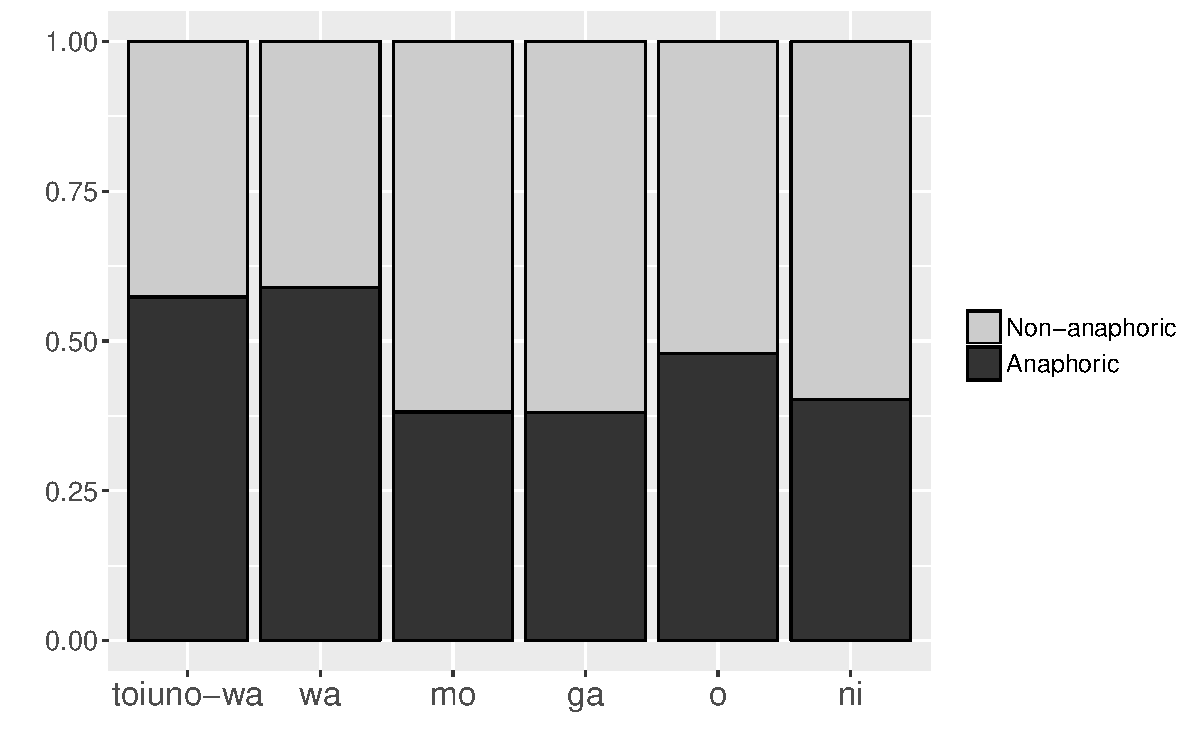
\includegraphics[width=0.8\textwidth]{figure/ParInfoStatus.pdf}
  \caption{Particle vs.\ information status (ratio)}
  \label{ParInfoStatusCTF}
\end{center}
\end{figure}

\begin{table}
 \begin{center}
 \tblcaption{\chd{The results of pairwise comparison among the least-squares means (information status)}}
 \label{Par:InfoStatusPar:LSMEANST}
 \begin{tabular}{lrrrrr}
 \toprule
 contrast      &    estimate &        SE & z.ratio & p.value & \\
 \midrule
  ga - o         & $-0.465$ & $0.149$ & $-3.120$ &  $0.022$ & * \\
  ga - wa        & $-0.748$ & $0.182$ & $-4.096$ & $<0.001$ & *** \\
  ga - toiuno-wa & $-0.659$ & $0.274$ & $-2.409$ &  $0.153$ &  \\
  o - wa         & $-0.282$ & $0.193$ & $-1.463$ &  $0.688$ &  \\
  o - toiuno-wa  & $-0.194$ & $0.282$ & $-0.688$ &  $0.983$ &  \\
  ni - wa        & $-0.661$ & $0.184$ & $-3.602$ &  $0.004$ & ** \\
  wa - toiuno-wa & $ 0.089$ & $0.293$ & $ 0.302$ &  $1.000$ &  \\
  wa - mo        & $ 0.759$ & $0.244$ & $ 3.107$ &  $0.023$ & * \\
 \bottomrule
 \end{tabular}
 \end{center}
\hfill{(0 $\le$ `***' $\le$ 0.001 $\le$ `**' $\le$ 0.01 $\le$ `*' $\le$ 0.05 `.' $\le$ 0.1 $\le$ ` ' 1)}
\end{table}

\begin{table}
	\begin{center}
	\tblcaption{Particle vs.~persistence}
	\label{ParPerNumT}
	\begin{tabular}{lrrrrrr}
	\toprule
	                  & \ci{toiuno-wa} & \ci{wa} & \ci{mo} & \ci{ga} & \ci{o} & \ci{ni} \\
	\midrule
	Persistent        & 45             & 107     & 53      & 209    & 175 & 184 \\
	                  & {\rt (66.2\%)} & {\rt (56.3\%)} & {\rt (44.9\%)} & {\rt (46.2\%)} & {\rt (51.5\%)} & {\rt (41.3\%)} \\
	Non-persistent    & 23             & 83     & 65      & 243    & 165 & 261 \\
	                  & {\rt (33.8\%)} & {\rt (43.7\%)} & {\rt (55.1\%)} & {\rt (53.7\%)} & {\rt (48.5\%)} & {\rt (58.7\%)} \\
	\midrule
	Sum               & 68             & 190     &  118    & 452    & 340 & 445 \\
%	                  & {\rt (100\%)} & {\rt (100\%)} & {\rt (100\%)} & {\rt (100\%)} & {\rt (100\%)} & {\rt (100\%)} \\
	\bottomrule
	\end{tabular}
	\end{center}
\end{table}

\begin{figure}
%\begin{minipage}{0.5\textwidth}
	\begin{center}
	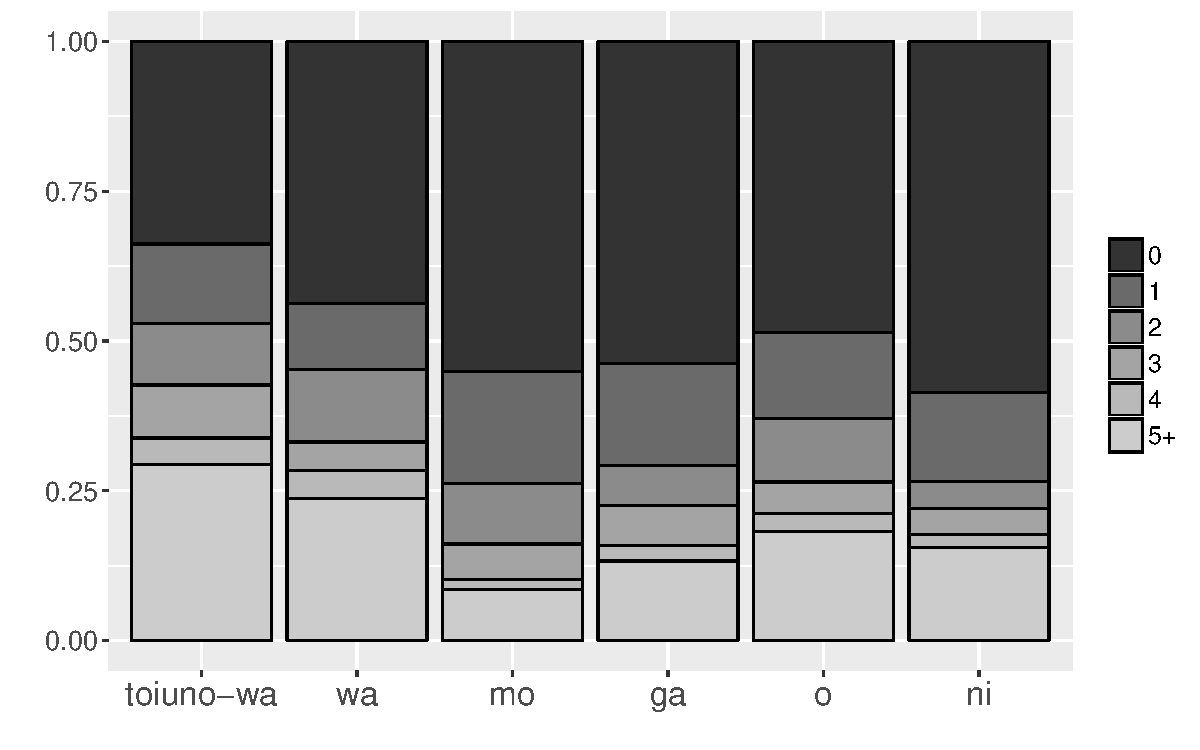
\includegraphics[width=0.8\textwidth]{figure/ParPerNum.pdf}
	\caption{Particle vs.\ \# of mention (ratio)}
	\label{ParPerNumF}
	\end{center}
\end{figure}
%\end{minipage}
%\begin{minipage}{0.5\textwidth}
%	\begin{center}
%	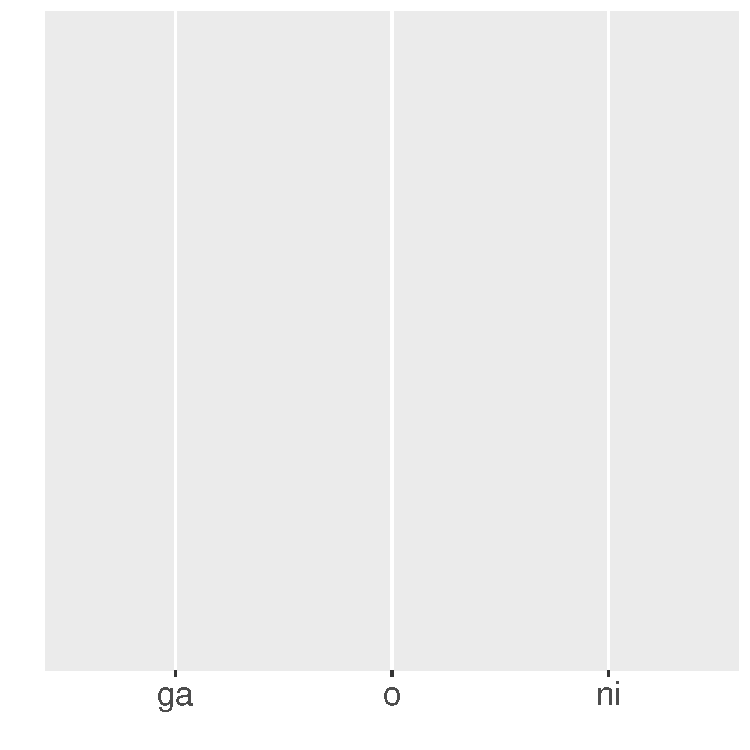
\includegraphics[width=0.95\textwidth]{figure/PerNumCasePar.pdf}
%	\caption{Case marker vs.\ \# of mention (ratio)}
%	\label{PerNumCaseParF}
%	\end{center}
%\end{minipage}

\begin{table}
 \begin{center}
 \tblcaption{\chd{The results of pairwise comparison among the least-squares means (persistence)}}
 \label{Par:PersistencePar:LSMEANST}
 \begin{tabular}{lrrrrr}
 \toprule
 contrast      &    estimate &        SE & z.ratio & p.value & \\
 \midrule
 ga - o         &  $-0.215$ & $0.146$ & $-1.473$ & $0.6817$ & \\
 ga - wa        &  $-0.349$ & $0.178$ & $-1.960$ & $0.3657$ & \\
 ga - toiuno-wa &  $-0.802$ & $0.281$ & $-2.856$ & $0.0491$ & * \\
 o - wa         &  $-0.134$ & $0.187$ & $-0.714$ & $0.9804$ & \\
 o - toiuno-wa  &  $-0.587$ & $0.287$ & $-2.044$ & $0.3171$ & \\
 o - ni         &  $ 0.440$ & $0.148$ & $ 2.978$ & $0.0345$ & * \\
 ni - wa        &  $-0.574$ & $0.180$ & $-3.189$ & $0.0179$ & * \\
 ni - toiuno-wa &  $-1.027$ & $0.282$ & $-3.642$ & $0.0037$ & ** \\
 wa - toiuno-wa &  $-0.453$ & $0.302$ & $-1.501$ & $0.6635$ & \\
 \bottomrule
 \end{tabular}
 \end{center}
 \hfill{(0 $\le$ `***' $\le$ 0.001 $\le$ `**' $\le$ 0.01 $\le$ `*' $\le$ 0.05 `.' $\le$ 0.1 $\le$ ` ' 1)}
\end{table}


Elements coded by so-called topic markers cannot be repeated as news, as shown in the hypothetical conversation between A and B in the following examples.
%
%	\ex. \ag. tozan-\EM{toiuno-wa} \\
%			mountain.climbing-\ab{quot}-\ci{wa} \\
%			`Mountain climbing is,'
%		\bg. ee yama-o nobot-te \\
%			\ab{fl} mountain-\ab{acc} climb-and \\
%			`(you) climb a mountain and'
%		\bg. tyoozyoo-ni tat-te \\
%			top-\ab{loc} stand-and \\
%			`(you) stand at the top of the mountain and'
%		\bg. soko-kara ee kudaru-toiu hitotu-no katee-ga aru-n-desu-keredomo \\
%			there-from \ab{fl} climb.down-\ab{quot} one-\ab{gen} process-\ab{nom} exist-\ab{nmlz}-\ab{cop}.\ab{plt}-though \\
%			`(you) climb down from there.' \hfill{(\code{S01F0151: 64.14-72.42})}
%		
%	\ex. hee, \{\EM{??tozan} / \}
%登山というのはえー山を登って
%頂上に立って
%そこからえー下るという一つの過程があるんですけれども (S01F0151: 64.14-72.42)
As in \Next and \NNext,
the \ci{toiuno-wa}-coded elements
\ci{mooningu thii} `morning tea'%
	\footnote{
	As discussed in \S \ref{Toiunowa},
	there are some formal variations of \ci{toiuno-wa};
	\ci{tteno-wa} is one of these variations.
	}
and \ci{eberesuto-kaidoo} `the Everest Trail'
cannot be repeated as news,
while the case-marker-coded elements \ci{kootya-ka koohii-ka} `tea or coffee', \ci{tibetto} `Tibet', \ci{nepparu} `Nepal', and \ci{kooeki-ro} `trading road'
can be repeated as news.
%
	\ex. \a.[A:] \ag. kono \EM{mooningu-thii-tteno-wa} \\
			this morning-tea-\ci{toiuno}-\ci{wa} \\
			`(In) this morning tea (time)'
		\bg. ma \EM{kootya-ka} \EM{koohii-ka-tteiuno-o} erab-eru-n-desu-keredomo \\
			\ab{fl} black.tea-or coffee-or-\ab{quot}-\ci{o} choose-can-\ab{nmlz}-\ab{plt}-though \\
			`(you) can choose tea or coffee.'
			 \hfill{(\code{S01F0151: 297.23-300.44})}
		\z.	
	\b.[B:] hee, \{\EM{??moo-ningu-thii(-wa)}/ \EM{kootya-ka koohii-o}\}\\
			Oh, \{morning tea/tea or coffee\}
	

%このモーニングティーってのはま紅茶かコーヒーかっていうのを選べるんですけれども (S01F0151: 297.23-300.44)
%
	\ex. \a.[A:] \ag. kono \EM{eberesuto-kaidoo-toiuno-wa} \\
			this Everest-road-\ab{quot}-\ci{wa} \\
			`This Everest Trail is'
		\bg. \EM{tibetto-to} \EM{nepaaru-no} \EM{kooeki-ro-ni}-mo nat-te ori-masi-te \\
			Tibet-and Nepal-\ab{gen} trade-road-for-also  become-and \ab{plt}-\ab{plt}-and \\
			`also used for trading between Tibet and Nepal.'
			 \hfill{(\code{S01F0151: 105.73-110.29})}
		\z.
	\b.[B:] hee, \{\EM{??eberesuto-kaidoo(-wa)}/\EM{tibetto-to}/\EM{nepaaru-to} / \EM{kooeki-ro-ni(-mo)}\}\\
			Oh, \{Everest Trail/Tibet/Nepal/trading road\}
	

%このエベレスト街道というのはチベットとネパールの交易路にもなっておりまして (S01F0151: 105.73-110.29)
%
As shown in \Next,
the element \ci{thii-taimu} `tea time' coded by the copula + \ci{kedo}%
	\footnote{
	Again there are some variations of this marker
	and I will discuss this in \S \ref{kedo}.
	}
or the \ci{wa}-coded element \ci{takai tokoro} `places of high elevation'
cannot be repeated as news,
while the \ci{ga}-coded elements can be repeated as news.
%
\ex. \a.[A:] \ag. de kono \EM{thii-taimu-nan-desu-keredomo} \\
		and this tea-time-\ab{nmlz}-\ab{cop}.\ab{plt}-though \\
		`And at this tea time,'
	\bg. kono hyookoo-no \EM{takai} \EM{tokoro-de-wa} koozanbyoo-toiu hizyooni \EM{kikennna} \EM{kanoosee-ga} aru-node \\
		this elevation-\ab{gen} high place-\ab{loc}-\ci{wa} altitude.sickness-\ab{quot} very dangerous possibility-\ab{nom} exist-because \\
		`this place of high elevation, there is a possibility of altitude sickness, so...'
	\bg. ee \EM{mizu-ga} hizyooni zyuuyooni nari-masu \\
		\ab{fl} water-\ab{nom} very important become-\ab{plt} \\
		`water is very important.'
		 \hfill{(\code{S01F0151: 339.78-349.56})}
	\z.
\b.[B:] hee, \{\EM{??thii-taimu}/\EM{??takai tokoro-de}/\EM{kikennna kanoosee-ga}/\EM{mizu-ga}\} \\
	Oh, \{tea time/on places of high elevation/the possibility of danger/water\}


%でこのティータイムなんですけれども
%この標高の高いところでは高山病という非常に危険な可能性があるので
%えー水が非常に重要になります (S01F0151: 339.78-349.56)
%
%僕らそのー新人で入った時っていうのは
%一応新人いー用にあまある程度残業代ってのが確保されてるらしいんですね (S05M1236: 393.59-401.15)
%
%On the other hand,
%\ci{mo}-coded elements can be repeated as news
%as shown in \Next.
%%
%\ex.\label{kosobo-tiiki-de-mo}
% \a.[A:]
% \ag. kono \EM{kosobo-tiiki-de-mo} \\
% 	this Kosovo-region-\ab{loc}-also \\
%	`Also in this Kosovo,'
% \bg. minzoku-hunsoo-ga okot-ta wake-de-gozaimasu-ga \\
% 	ethnic-conflict-\ci{ga} happen-\ab{past} reason-\ab{cop}-\ab{plt}-though \\
%	`ethnic conflicts occurred, and...'
%	\hfill{(\code{S00M0199: 163.04-165.91})}
% \z.
% \b.[B:] hee, \{$^{ok}$kosobo-tiiki-de(-mo)/minzoku-hunsoo-ga\} \\
% 	Oh, \{(also) in Kosovo/ethnic conflicts\}.
%
%このコソボ地域でも
%民族紛争が起こった訳でございますが
% (S00M0199: 163.04-165.91)
%
%According to Figure \ref{TopParInfoStatusF} and Table \ref{TopParInfoStatusT},
%more than half of the \ci{mo}-coded elements are new,
%and, according to Figure \ref{PerNumTopParF} and Table \ref{PerNumTopParT},
%approximately half of the \ci{mo}-coded elements are non-persistent.
%Based on our criteria for topic,
%\ci{mo}-coded elements are not topics.
%The characteristics of elements coded by \ci{mo} `also' will be discussed in \S \ref{Mo}.
%Basically \ci{mo} codes an element
%in addition to some set that has already been introduced.

As indicated in Table \ref{ParInfoStatusT} and will be discussed below,
brand-new elements can never be coded by topic markers;
they can never be assumed to be shared between the speaker and the hearer.
Non-anaphoric elements coded by topic markers are
inferable, declining, or unused,
as will be discussed in the following sections.
%as has been pointed out in \citeA{kuno73} and as has been discussed in \S \ref{BackSecTopic}.
For example,
as in \Next,
it is unacceptable for topic markers to code brand new elements \ci{oozei-no hito} `many people' out of the blue.
% without assuming that the hearer can identify which girl the speaker is talking about.%
%	\footnote{
%	As discussed in \S \ref{TopZero} and \S \ref{FocZero},
%	the agent-like argument of transitive clauses can be zero-coded if it is a topic,
%	while it cannot if it is (part of) a focus.
%	Hence the zero markers that code \ci{oozei-no hito} `many people' in \Next and \ci{otoosan} `father' in \NNext are unambiguously interpreted as topic zero marker.
%	}
%
\exg.
 *\EM{oozei-no} \EM{hito-wa} paathii-ni ki-masi-ta \\
  many-\ab{gen} person-\ci{wa} party-\ab{dat} come-\ab{plt}-\ab{past} \\
  `Speaking many people, they came to the party.'
    \hfill{\cite[~45]{kuno73}}
% \bg. *dareka-\EM{wa} byooki-desu \\
%       somebody-\ci{wa} sick-\ab{cop}.\ab{plt}\\
%       `Speaking of somebody, he is sick.'
%       \hfill{(ibid.)}

Similarly, it is unacceptable for other topic markers to code these elements, whereas \ci{ga} can code them.
%
\exg.
 \EM{oozei-no} \EM{hito-\{??{toiuno-wa}/??da-kedo/??{\O}/ga\}} paathii-ni ki-masi-ta \\
 many-\ab{gen} person-{\{\ci{toiuno-wa}/\ab{cop}-\ci{though}/{\O}/\ci{ga}\}} party-\ab{dat} come-\ab{plt}-\ab{past} \\
 `Many people came to the party.'
% \bg. dareka-\{??{toiuno-wa}/??wa/??da-kedo/??{\O}/ga\} ki-masi-ta-ne \\
%       somebody-\{\ci{toiuno-wa}/\ci{wa}/\ab{cop}-\ci{though}/{\O}/\ci{ga}\} come-\ab{plt}-\ab{past}-\ab{fp} \\
%       `Somebody came.'


%\exg. a! \label{onnanoko}\EM{onnanoko-\{??{toiuno-wa}/??wa/??da-kedo/??{\O}/ga\}} henna boosi kabut-temasu-yo \\
% oh! girl-\{\ci{toiuno-wa}/\ci{wa}/\ab{cop}-\ci{though}/{\O}/\ci{ga}\} weird hat wear-\ab{prog}.\ab{plt}-\ab{fp} \\
% `A girl is wearing a red hat.' 

%Although it is possible to interpret \Last as ``girls in general wear red hats,''
%it is otherwise unacceptable.
While \ci{oozei-no hito} `many people' in \Last was unanchored in terms of \citeA{prince81},
\ci{taroo-no otoosan} `Taro's father' in \Next is anchored.
The element coded by a topic marker is still not acceptable in an out-of-the-blue context.
%
\exg. a! \EM{taroo-no} \EM{otoosan-\{??{toiuno-wa}/??wa/??da-kedo/{\O}\}} asoko-de tabako sut-teru-yo \\
 oh! Taro-\ab{gen} father-\{\ci{toiuno-wa}/\ci{wa}/\ab{cop}-\ci{though}/{\O}\} there-\ab{loc} cigarette smoke-\ab{prog}.\ab{plt}-\ab{fp} \\
 `Taro's father is smoking over there.'

Therefore, topic markers in Japanese are sensitive to the given-new taxonomy rather than definiteness and identifiability.%
 \footnote{
 I suppose that the zero particle is acceptable
 because the zero particle in this case is ambiguous between topic and focus coding.
 }

Finally, as will be discussed in detail in \S \ref{TopZero},
an element coded by a zero particle ({\O}) that precedes other arguments and is uttered in a coherent intonation contour
cannot be repeated as news and hence considered to be presupposed to be shared.
\ex. \label{mouse}Context: Y and H are roommates,
	who are bothered by a mouse running around their room
	and eating their leftovers.
	The cat they keep finally caught the mouse while H was out.
	When H is back, Y wants to let H know this news.
	\ag.[Y:] \EM{nezumi-\O} neko-ga tukamae-ta-yo \\
		nezumi-{\O} cat-\ci{ga} catch-\ab{past}-\ab{fp} \\
		`The cat caught (the) mouse.'
	\b.[H:] hee, \{??nezumi, neko(-ga)\} \\
	  Oh, \{mouse, cat(-\ci{ga})\}
	  \hfill{(=\ref{FrameworkExMouse} in \S \ref{FrameworkTopic})}


In the following sections,
I analyze each topic marker in detail.

%%----------------------------------------------------
\subsection{\textit{Toiuno-wa}}\label{Toiunowa}

In this section
I will show that \ci{toiuno-wa} codes elements of referents
which are evoked
through explicit or implicit introduction of the elements or
availability in the universe of discourse.

There are phonetic variations of \ci{toiuno-wa}:
\ci{(t)teno-wa}, \ci{t(y)uuno-wa}, \ci{teiuno-wa}, etc.
I put them into the same category as \ci{toiuno-wa} and assume that they are the same
except for stylistic difference.


%%----------------------------------------------------
\subsubsection{Evoked elements tend to be coded by \textit{toiuno-wa}}

\ci{Toiuno-wa} typically codes evoked elements.
As exemplified in \Next and \NNext,
the antecedents of the \ci{toiuno-wa}-coded elements,
\ci{un} `luck' in \Next and \ci{tiryoo-hoo} `treatment methods' in \NNext,
are mentioned in the immediately preceding contexts.
%
\ex.
 \ag. syokugyoo-ni taisite-no \EMi{un}-toiu koto-o tyotto o-hanasi si-tai-to omoi-masu \\
		job-to towards-\ab{gen} luck-\ab{quot} thing-\ci{o} a.bit \ab{plt}-talk do-want-\ab{quot} think-\ab{plt} \\
		`I'd like to speak a bit about the role of luck in one's career.'
 \bg. de \EM{un-toiuno-wa} maa iroirona un-ga aru-to omou-n-desu-keredomo \\
 	then luck-\ci{toiuno-wa} \ab{fl} various luck-\ci{ga} exist-\ab{quot} think-\ab{nmlz}-\ab{plt}-though \\
	`I guess there are various kinds of lucks...'
	\hfill{(\code{S01F0038: 0.53-8.70})}
%職業に対しての運ということをちょっとお話ししたいと思います
%で運というのはまー色々な運があると思うんですけれども
%(S01F0038: 0.53-8.70)

\ex. \ag. de sono byooki-wa gen'in-ga humee-de \\
	and that disease-\ci{wa} source-\ci{ga} unknown-\ab{cop} \\
	`And the source of that disease was unknown, and'
	\bg. \EMi{tiryoo-hoo}-mo kakuritu-si-tei-mas-en-desi-ta \\
		treatment-method-also establish-do-\ab{pfv}-\ab{plt}-\ab{neg}-\ab{plt}-\ab{past} \\
		`The treatment methods had not been established.'
	\bg. sono \EM{tiryoo-hoo-toiuno-wa} yuiitu ... suteroidozai-de sinkoo okur-aseru koto-dake-desi-ta \\
		that treatment-method-\ci{toiuno-wa} only ... steroid-by progress delay-\ab{caus} thing-only-\ab{plt}-\ab{past} \\
		`The only way to treat is just to delay the progress of the disease using steroid, which I cannot use.' \hfill{(\code{S02F0100: 294.39-308.12})}

%でその病気は原因が不明で治療法も確立していませんでした
%その治療法というのは唯一私が使うことのできないステロイド剤で進行遅らせることだけで (S02F0100: 294.39-308.12)

Non-anaphoric elements coded by \ci{toiuno-wa} are considered to be evoked
through implicit introduction of an element or by the physical context.
In \Next,
\ci{supootu-kansen} `sport watching' is non-anaphoric
but the speaker mentioned that he watched a world title match.
Thus `sport watching' is considered to be evoked
when the speaker mentioned `sports watching' with \ci{toiuno-wa} coding in line c.
%
\ex. \ag. ee \EMi{sekai-taitoru-sen-o-desu-ne} ee \EMi{terebi-de} \EMi{mi-masi-ta} \\
		\ab{fl} world-title-fight-\ci{o}-\ab{plt}-\ab{fp} \ab{fl} TV-by watch-\ab{plt}-\ab{past} \\
		`(My friend and I) watched a world title match on TV.'
	\b. ...
	\bg. watasi-zisin gu -wa ee amari koo \EM{supootu-kansen-teiunowa} tyotto si-nakat-ta-n-desu-ne \\
		\ab{1}\ab{sg}-self \ab{frg} -\ci{wa} \ab{fl} not.really \ab{fl} sport-watching-\ci{toiuno-wa} \ab{fl} do-\ab{neg}-\ab{past}-\ab{nmlz}-\ab{plt}-\ab{fp} \\
		`I myself hadn't watched any kinds of sports.' \hfill{(\code{S01M0182: 52.77-79.62})}
%	
%えー世界タイトル戦をですねえーテレビで見ました
%...
%私自身ぐはえーあまりこうスポーツ観戦ていうのはちょっとしなかったんですね (S01M0182: 52.77-79.62)

Similarly, in \Next,
\ci{taitoru} `title (in piano competitions)' is a non-anaphoric element
but the speaker was talking about `awards' in the preceding context
and `title' can be considered to have been evoked at the time of utterance \Next[e].
%
\ex. \a. I have been participating in various piano competitions
	\b. So far the best award I received was the fourth best place in the China-Japan International Competition.
	\b. Beyond that, I would like to receive higher awards.
	\bg. ano doositemo kore-wa yappari piano-o kokorozasu mono-ni totte-wa \\
		\ab{fl} anyhow this-\ci{wa} anyway piano-\ci{o} orient people-for in.terms.of-\ci{wa} \\
		`This, for those who want to make name as a pianist,'
	\bg. kono \EM{taitoru-tteiuno-wa} sugoku ookii-node \\
		this title-\ci{toiuno-wa} very big-because \\
		`titles matter a lot, so...'
\hfill{(\code{S00F0209: 507.13-529.76})}
%
%やはりあの今まで受けたコンクールの最高順位が
%あのま日中友好国際音音楽コンクールっていうのがあって
%それがまー一般のピアノ部門で四位で奨励賞だったんですね
%でそれを超えてあの三位以内に入賞することがまず一つで
%あのどうしてもこれはやっぱりピアノを志す者にとっては
%このタイトルってのは凄く大きいので (S00F0209: 507.13-529.76)

In another example like \Next,
\ci{toiuno-wa}-coded elements are considered to be evoked through ``common sense''.
\Next is the beginning of the talk
but the speaker mentions \ci{ningen} `human being' with \ci{toiuno-wa} coding.
This is because
people can always talk about human beings even in out-of-the-blue contexts.
Therefore, ``human beings'' are always available as topic.
\ci{Tuuno-wa} is a variation of \ci{toiuno-wa}.
%the human being is always evoked through the physical context.
%
\exg.\label{ExNingenToiunowa}\EM{ningen-tuuno-wa} hizyooni ano umaku deki-teru doobutu-da-to omoi-masu-ne \\
	human-\ci{toiuno-wa} very \ab{fl} well created-\ab{pfv} animal-\ab{cop}-\ab{quot} think-\ab{plt}-\ab{fp} \\
	`I think that human beings are well-created.' \\
 \hfill{(\code{S02M1698: 6.99-11.00})}
%
%人間つうのは非常にあのうまくできてる動物だと思いますね (S02M1698: 6.99-11.00)

Readers might think that \Last is acceptable because `human being' is generic rather than evoked in the physical context.
However, I do not employ this account for the following two reasons:
(i) being generic is a characteristic across all \ci{toiuno-wa}-coded elements (see \S \ref{Par:Topic:Toiunowa:Other}), and
(ii) even though the elements are generic, some elements are still difficult to be coded by \ci{toiuno-wa} in the beginning of speeches.
%Let us discuss example \Next, which is at the very beginning of a speech about Kosovo conflicts.
\chd{Let us discuss example \Next,
which is at the very beginning of a speech about travel to Hawaii.}
%
\exg.\label{Par:Toiunowa:Ex:Hawaii}teema-wa hawai-too-no sizen-no subarasisa-to tabi-no tanosisa-nituite-desu \\
   theme-\ci{wa} Hawaii-island-\ab{gen} nature-\ab{gen} splendor-and travel-\ab{gen} fun-about-\ab{cop} \\
   `The topic (of this talk) is about the splendor of Hawaii nature and fun of traveling.'
 \hfill{(\code{S00F0014: 0.30-6.08})}
%テーマはハワイ島の自然の素晴らしさと旅の楽しさについてです
%%
%\ex.\label{ExKosovo}
% \ag. ee \ci{kosobo-mondai}-ni-tuite \\
%	\ab{fl} Kosovo-problem-on-about \\
%	`On Kosovo conflicts.'
% \bg. ee ima-kara tyoodo ee iti-nen-hodo-mae-ni nari-masu-ne \\
% 	\ab{fl} now-from exactly \ab{fl} one-year-ago-about-to become-\ab{plt}-\ab{fp} \\
%	`From now, it was exactly a year ago...'
%	\hfill{(\code{S00M0199: 0.24-10.50})}
%%えーコソボ問題について
%%えー今からちょうどえー一年程前になりますね
%% (S00M0199: 0.24-10.50)

\chd{In this example,
the speaker did not choose to code `the splendor of Hawaii nature and fun of traveling' with \ci{toiuno-wa}.
It is harder to code this with \ci{toiuno-wa} than `human being' because
it is not always available as topic
even though `the splendor of Hawaii nature and fun of traveling'
is generic.}
%The sentence itself is natural if \ci{ni-tuite} is replaced with \ci{toiuno-wa}.
%(In that case, \Last[a-b] are considered to be a single coherent sentence.)
%However, it is slightly unnatural without introducing `Kosovo conflict'
%in the preceding discourse.
Therefore,
I argue that the acceptability of \ci{toiuno-wa} coded `human being' without introduction of human beings in \LLast is possible
because it is always available as topic,
not because it is generic.


%%----------------------------------------------------
\subsubsection{Declining or inferable elements tend not to be coded by \textit{toiuno-wa}}\label{Toiuno-waInfSemiActUnuse}

There are a few examples
where \ci{toiuno-wa} codes inferable elements.
In \Next,
the speaker explains why she came to Iran and describes the middle school there.
The climate in Iran has not been mentioned before \Next[c],
but is still coded by \ci{toiuno-wa}.
The climate in Iran is neither implicitly introduced nor available as universal topic.
\ex. \label{IranClimate}
 \a. (The speaker moved to Iran when she was a middle school student.)
 \b. (The school for Japanese students in Iran was small but she had a lot of fun there.)
 \bg. eeto iran-no \EM{kikoo-tteiuno-wa} tomokaku kansoo si-tei-masi-te \\
 	\ab{fl} Iran-\ab{gen} \ci{climate-toiuno-wa} at.any.rate dry do-\ab{prog}-\ab{plt}-and \\
	`Uh, the climate in Iran was very dry...'
	\hfill{(\code{S03F0072: 178.31-181.65})}
%えーとイランの気候っていうのはともかく乾燥していまして
% (S03F0072: 178.31-181.65)
%

Similarly, in \Next[c],
the speaker is going to talk about a dog his family kept.
The speaker begins with the explanation why the dog came to his house.
The element \ci{keei} `background (of why the dog came)' is coded by \ci{toiuno-wa},
although \ci{keei} has not been explicitly mentioned in the preceding context.
%
\ex.
 \a. (The speaker talks about a dog his family kept.)
 \b. (After the death of the previous dog they kept, the dog he is going to talk about joined his family.)
 \bg. e uti-ni ki-ta \EM{keei-toiuno-wa} \\
 	\ab{fl} home-to come-\ab{past} background-\ci{toiuno-wa} \\
	`The background of how the dog came to our house is'
 \bg. ma sono zyuui-san-no syookai-nan-desu-keredomo \\
 	\ab{fl} that vet-\ab{hon}-\ab{gen} introduction-\ab{nmlz}-\ab{cop}.\ab{plt}-though \\
	`(through) the introduction of that vet...'
	\hfill{(\code{S02M0198: 141.97-146.92})}
%えうちに来た経緯というのは
%まその獣医さんの紹介なんですけれども
% (S02M0198: 141.97-146.92)


On the other hand,
there are some cases where it is unnatural for \ci{toiuno-wa} to code inferable elements.
For example, in \Next[c],
the element \ci{hikoozyoo} `airport' cannot naturally be coded by \ci{toiuno-wa},
which is originally coded by \ci{wa}.
The airport is inferable because the speaker has already mentioned flying to Lukla.
\ex.
%
%		\ag. hikooki-de ee hyookoo 2600 meetoru-no rukura-to iu mura-ni mazu tobi-masu \\
%			airplane-by \ab{fl} elevation 2600 meter-\ab{gen} Lukla-\ab{quot} call village-to first fly-\ab{plt} \\
	\a. To start Himalaya trekking, you first fly to a village called Lukla whose elevation is 2600 meters.
%		\bg. soko-kara ee torekkingu-o kaisi-itasi-masi-ta \\
%			that-from \ab{fl} trekking-\ab{acc} start-do-\ab{plt}-\ab{past} \\
	\b. From that village, we started trekking.
	\bg. sono rukura-no mura-nan-desu-ga \\
		that Lukla-\ab{gen} village-\ab{nmlz}-\ab{plt}-though \\
		`Regarding that Lukla village,'
	\bg. \EM{hikoozyoo-\{wa}(/??-\EM{toiuno-wa})\} hontooni yama-no naka-ni ari-masi-te \\
		airport-\ci{wa}(/-\ci{toiuno-wa}) really mountain-\ab{gen} inside-in exist-\ab{plt}-and \\
		`the airport is really in a mountainous area.'
	\hfill{(\code{S01F0151: 179.50-191.39})}
%飛行機でえー標高二千六百メートルのルクラという村にまず飛びます
%そこからえートレッキングを開始いたしました
%そのルクラの村なんですが
%飛行場は本当に山の中にありまして (S01F0151: 179.50-191.39)

I speculate that the different acceptabilities of \ci{toiuno-wa} among \ref{IranClimate}, \LLast, and \Last are due to different statuses in the given-new taxonomy or the accessibility of the elements;
`the climate' in \ref{IranClimate} and `the background' in \LLast are more general terms and are more easily accessible
than `the airport' in \Last.
Note that this does not contradict, but rather is consistent with, the Semantic Map Connectivity Hypothesis \ref{SemanticMapHypIS}.
Since the given-new taxonomy scale is continuous,
the boundary between evoked and inferable is blurred, and
among the inferable elements in these examples,
`the climate' of Iran in \ref{IranClimate} and `the background' in \LLast are easier to access than `the airport' in \Last.
This is consistent with the nature of the conceptual space,
although the boundary is drawn clearly in the semantic map in Table \ref{ParInfoStatusT}
for the purpose of presentation.

It is unnatural when \ci{toiuno-wa} codes declining elements.
The degree of how a referent is declining is difficult to calculate from the corpus.
Apparently, it does not simply correspond to the distance between an element and its antecedent,
but the intervention of (an)other topic(s) seems to be more relevant.
For example,
a copula followed by \ci{kedo} codes declining or unused elements, as will be shown in \S \ref{kedo}.
In \Next[g],
it codes a declining element rather than unused element
because the element has already been introduced in line a.
In line a, two potential topics `fame' and `job' are introduced.
The speaker talks about `fame' first and moves on to `job' in line g.
It is fair to assume that the topic `job' is intervened by another topic `fame'.
When the element `job' is retrieved as a current topic in line g,
it is coded by a copula followed by \ci{keredomo} `though',
a variation of \ci{kedo}.
However,
this marker cannot be replaced with \ci{toiuno-wa}.
%
\ex.\label{sigoto}
 \a. I have two goals: one is for \EMi{fame} and the other is for \EMi{\EMi{job}}.
 \b. Concerning \EMi{fame},
 \b. I have been participating in various piano competitions
 \b. So far the best award I received was the fourth best play in the China-Japan International Competition.
 \b. Beyond that, I would like to receive higher awards.
 \b. Titles matter a lot for pianists, so I will work hard.
 \bg. de ato-wa \EM{sigoto-no} \EM{bubun-\{nan-desu-keredomo/(??toiuno-wa)\}} \\
 	then remaining-\ci{wa} job-\ab{gen} part-\{\ab{nmlz}-\ab{cop}.\ab{plt}-though/\ci{toiuno-wa}\} \\
	`Concerning the other one, job,'
 \b. to receive higher wages...
\hfill{(\code{S00F0209: 495.77-539.19})}
%
%これからのあの目標っていうのがありまして
%まそれは大きく分けて二つあるんですけども
%ま名声の部分と仕事っていう部分がありまして
%一番目の名声の部分は
%やはりあの今まで受けたコンクールの最高順位が
%あのま日中友好国際音音楽コンクールっていうのがあって
%それがまー一般のピアノ部門で四位で奨励賞だったんですね
%でそれを超えてあの三位以内に入賞することがまず一つで
%あのどうしてもこれはやっぱりピアノを志す者にとっては
%このタイトルってのは凄く大きいので
%あのやってきたいです
%で後は仕事の部分なんですけれども
%あの一回のギャランティーがえーと勿論アップするように
% (S00F0209: 495.77-539.19)


%\begin{figure}
%\begin{minipage}{0.5\textwidth}
%	\begin{center}
%	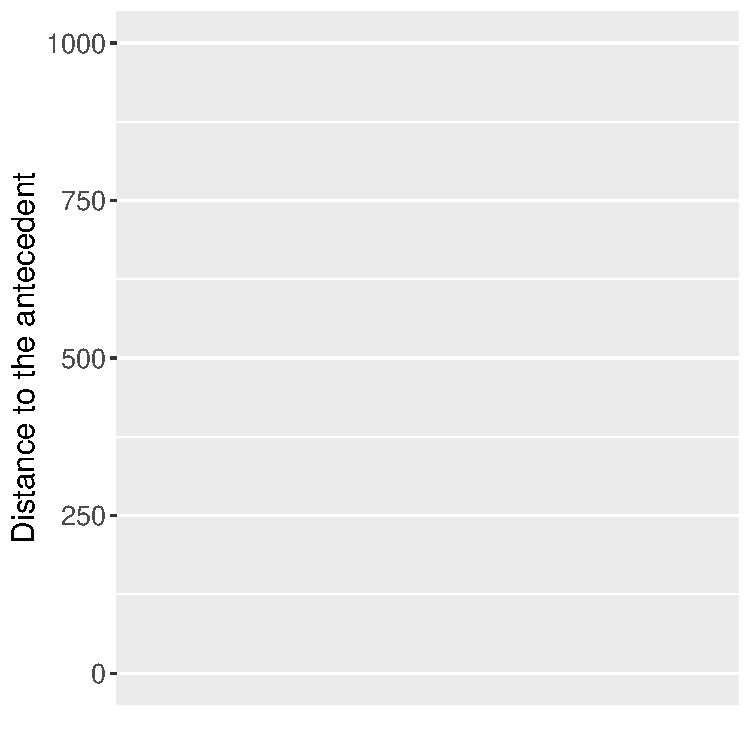
\includegraphics[width=0.95\textwidth]{figure/AnaRelDistTop.pdf}
%	\caption{}
%	\label{AnaRelDistTopF}
%	\end{center}
%\end{minipage}
%\begin{minipage}{0.5\textwidth}
%	\begin{center}
%	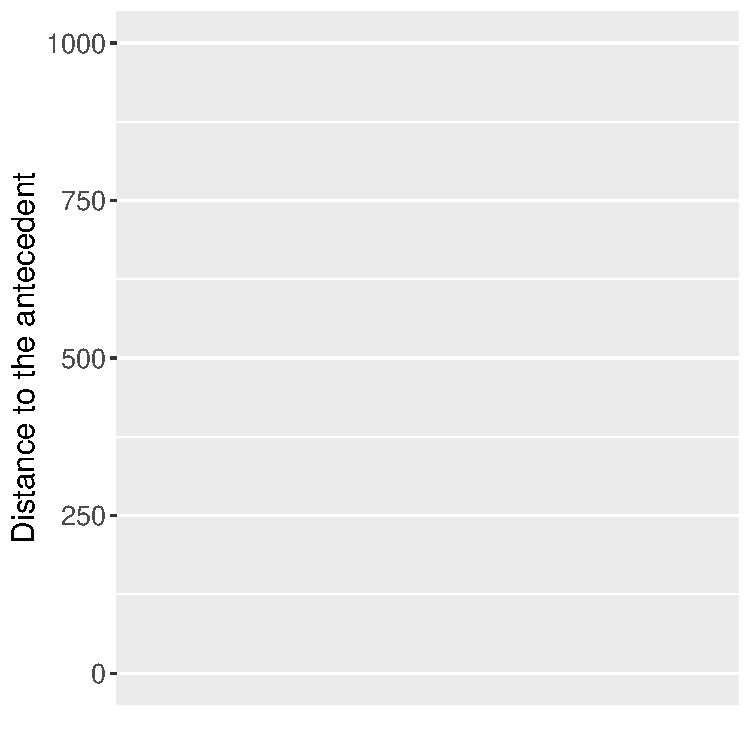
\includegraphics[width=0.95\textwidth]{figure/AnaRelDistCase.pdf}
%	\caption{}
%	\label{AnaRelDistCaseF}
%	\end{center}
%\end{minipage}
%\end{figure}



\ci{Toiuno-wa} cannot code elements that have not been established as topic.
In \Next,
although `tea time' is introduced in line b,
it does not appear to be established enough as topic,
which makes \ci{toiuno-wa} unnatural in line d;
the original marker is a copula followed by \ci{keredomo}.
%
\ex.\label{thii-taimu}
 \a. While we trek on the Everest Trail, the cook made us lunch on the way,
 \b. in addition, there is tea time and we can take a break while we climb the mountain,
 \b. so, we walked without feeling that we were in a big group.
 \bg. de kono \EM{thii-taimu-nan-desu-\{keredomo/(??toiuno-wa)\}} \\
		and this tea-time-\ab{nmlz}-\ab{cop}.\ab{plt}-\{though/toiuno-wa\} \\
		`And at this tea time,'
 \bg. kono hyookoo-no {takai} {tokoro-de-wa} koozanbyoo-toiu hizyooni {kikennna} {kanoosee-ga} aru-node \\
		this elevation-\ab{gen} high place-\ab{loc}-\ci{wa} altitude.sickness-\ab{quot} very dangerous possibility-\ci{ga} exist-because \\
		`this place of high elevation, there is a possibility of altitude sickness, so...'
 \bg. ee {mizu-ga} hizyooni zyuuyooni nari-masu \\
		\ab{fl} water-\ci{ga} very important become-\ab{plt} \\
		`water is very important.'
		 \hfill{(\code{S01F0151: 323.00-349.56})}
%途中でえー勿論お昼御飯もキッチンスタッフが作ってくれたり
%後はティータイムって言って
%途中でちょっとブレークする時間もあるんですけれども
%えーかなりえーそういうツアーで来ているっていう印象をそんなに与えないで
%えー歩くことができました
%でこのティータイムなんですけれども
%この標高の高いところでは高山病という非常に危険な可能性があるので
%えー水が非常に重要になります (S01F0151: 323.00-349.56)

These subtle differences of acceptability of \ci{toiuno-wa} cannot be captured simply by counting numbers.
However, they are clear from the acceptability judgements.

Unused elements also cannot be coded by \ci{toiuno-wa}.
It is very difficult to find unused elements
because of the nature of our corpus;
each speaker gave a speech in front of people s/he does not know
and there are few things the speaker can assume to be shared with the hearer(s).
However, constructed examples like \Next clearly show that \ci{toiuno-wa} cannot code unused elements.
%
\ex. \label{FacebookParty}Context: According to Facebook, both A and B are going to a party tomorrow. But they have not seen each other for a week. A sees B in a classroom and talks to B:
	\a.[A:] asita-no \EM{paathii-\{da-kedo/??toiuno-wa\}} nan-zi-kara-na-no \\
		tomorrow-\ab{gen} party-\{\ab{cop}-though/\ci{toiuno-wa}\} what-o'clock-from-\ab{cop}-\ab{q} \\
		`What time does tomorrow's party start?' 

Note that if the element `party' has already been introduced into the discourse, \ci{toiuno-wa} can code it.
This is shown in \Next[A].%
	\footnote{
	In this example, I am using \ci{tteiuno-wa} instead of \ci{toiuno-wa}
	simply because this hypothetical utterance is casual;
	\ci{tteiuno-wa} is more casual than \ci{toiuno-wa}.
	\ci{Toiuno-wa} sounds too formal in this utterance.
	}
\ex. \label{Party}Context: A and B are having a conversation. B mentioned tomorrow's party, which A knows that both A and B are going to.
	\ag.[A:] sono \EM{paathii-\{??da-kedo/tteiuno-wa\}} nan-zi-kara-na-no \\
		that party-\{\ab{cop}-though/\ci{toiuno-wa}\} what-o'clock-from-\ab{cop}-\ab{q} \\
		`What time does tomorrow's party start?' 


%%----------------------------------------------------
\subsubsection{Further characteristics of \textit{toiuno-wa}-coded elements}\label{Par:Topic:Toiunowa:Other}

Statements about \ci{toiuno-wa}-coded elements tend to represent the general characteristics of the referents,
as has been pointed out in \citeA{masuoka87,masuoka08}.
Masuoka argues that \ci{toiuno-wa}-coded elements only accompany individual-level predicates (in his term, property predicates).
This is clearly shown in the contrast between \Next[a] and \Next[b] (repeated from \ref{ExSatiko}) in \S \ref{Back:GeneralChar:Toiunowa}.
Whereas the stage-level predication \Next[a] does not allow \ci{toiuno-wa},
the individual-level predication \Next[b] does allow \ci{toiuno-wa}.
%
\ex.
\ag. *satiko-\EM{toiuno-wa} uso-o tui-ta \\
     Sachiko-\ci{toiuno-wa} lie-\ci{o} commit-\ab{past} \\
     `Sachiko lied.'
     \hfill{\cite[96]{masuoka12}}
\bg. satiko-\EM{toiuno-wa} uso-tuki-da \\
     Sachiko-\ci{toiuno-wa} lie-commiter-\ab{cop} \\
     `Sachiko is a liar.'
     \hfill{(Constructed)}

In our corpus,
most examples of \ci{toiuno-wa} also accompany individual-level predication
rather than stage-level predication.
In \Next,
the speaker is talking about the general characteristics of puppies.
%
\exg. \EM{koinu-toiuno-wa} dono syurui-demo hizyooni ano neru-no-ga tokui-desu-ne \\
 puppy-\ci{toiuno-wa} which kind-also very \ab{fl} sleep-\ab{nmlz}-\ci{ga} good.at-\ab{cop}.\ab{plt}-\ab{fp} \\
 `Puppies are, no matter what kind, good at sleeping.'
 \hfill{(\code{S02M1698: 166.62-170.59})}
%小犬というのはどの種類でも非常にあの寝るのが得意ですね
% (S02M1698: 166.62-170.59)

The explanation for this requires further investigation.

%As exemplified in the contrast between \Next[b] and \Next[b$^{\prime}$],
%\ci{toiuno-wa} can be used when the statement is about the usual event for the cat,
%while it cannot when the statement is about the event that happened only once.
%%
%\ex.
% \a. I had a cat when I was small.
% \bg. sono \EM{neko-toiuno-wa} yoku mado-no soto-o mi-tei-masi-ta \\
% 	that cat-\ci{toiuno-wa} often window-\ab{gen} outside-\ci{o} look-\ab{prog}-\ab{plt}-\ab{past} \\
%	`The cat was often looking at the outside of the window...'
% \bg.[b$^{\prime}$.] aru hi watasi-ga gakkoo-ni iku toki sono \EM{neko-\{??toiuno-wa/wa\}} mado-no soto-o mi-tei-masi-ta \\
% one day \ab{1}\ab{sg}-\ci{ga} school-to go when that cat-\{\ci{toiuno-wa}/\ci{wa}\} window-\ab{gen} outside-\ci{o} look-\ab{prog}-\ab{plt}-\ab{past} \\
% `One day, when I was going to school, the cat was looking at the outside of the window...'
 


%\ex. 
% \a. kitee-ga ari-masi-te \\
% 	rule-\ci{ga} exist-\ab{plt}-and \\
%	`There is a rule (for collecting debts from people),'
% \b. n o sono \EM{kaisyuu-rinri-kitee-tteiuno-wa} \\
% 	\ab{fl} \ab{fl} collect-ethic-rule-\ci{toiuno-wa} \\
%	`the rule'
% \b. ironna koomoku-de takusan ume-rare-te-desu-ne \\
% 	various point-with a.lot fill-\ab{pass}-\ab{prog}-\ab{plt}-\ab{fp} \\
%	`is filled with a lot of points...'
%	\hfill{(\code{S00M0221: 473.74-481.94})}
%規定がありまして
%んおその回収倫理規定っていうのは
%色んな項目でたくさん埋められててですね
% (S00M0221: 473.74-481.94)





%%----------------------------------------------------
\subsection{\textit{Wa}}\label{Wa}

\ci{Wa} codes inferable elements in addition to evoked elements.
Overall, the referents of \ci{wa}-coded elements are assumed to be
borne in the hearer's mind at the time of utterance,
or can be easily accommodated to the assumption.

%%----------------------------------------------------
\subsubsection{Evoked and inferable elements tend to be coded by \textit{wa}}

As exemplified in the following examples,
\ci{wa} can code evoked elements.
In \Next,
`chelow kebab' is mentioned in line a,
and it is mentioned again in lines b and g.
The second and the third mentioned elements are coded by \ci{wa}.
%
\ex.\label{kebab}
 \a. There is a dish called \EMi{chelow kebab}.
 \bg. de \EM{sore-wa} eeto gohan-ni eeto bataa-o maze-te \\
 	and that-\ci{wa} \ab{fl} rice-to \ab{fl} butter-\ci{o} mix-and \\
	`That, you mix rice with butter...'
 \b. on top of that you put spice,
 \b. on top of that you put mutton,
 \b. you mix it and eat it.
 \b. There were many dishes of this kind.
 \bg. \ci{sore-wa} kekkoo sonnani hituzi-no oniku-no kusasa-mo naku-te \\
 	that-\ci{wa} to.some.extent not.really sheep-\ab{gen} meat-\ab{gen} smell-also not.exist-and \\
	`It did not have smell of mutton...'
 \b. I thought it was delicious.
 \hfill{(\code{S03F0072: 446.03-471.72})}
%チェロカバブというのがありまして
%でそれはえーと御飯にえーとバターを混ぜて
%その上に香辛料を振って
%その上に羊のお肉が乗っていて
%それをこう混ぜて
%ぐちゃぐちゃに混ぜて食べるという
%えーとお料理があのー多かったんですけれども
%それは結構そんなに羊のお肉の臭さもなくて
%あのーおいしいなって思って
% (S03F0072: 446.03-471.72)

Also in \Next,
`the result of the medical exam' is mentioned in line b,
and it is mentioned again in line c, which is coded by \ci{wa}.
%
\ex.\label{kensakekka}
 \ag. de sosite is-syuu anoo zibun-de-mo odoroku-hodo reeseeni \\
 	then and one-week \ab{fl} self-for-also be.surprised-degree calmly \\
	`For a week, surprisingly calmly,'
 \bg. kensa-no \EM{kekka}-o mati-masi-ta \\
 	exam-\ab{gen} result-\ci{o} wait-\ab{plt}-\ab{past} \\
	`I was waiting for the result of the medical exam.'
 \bg. nde sono kensa-no \EM{kekka-wa} hutuu-no hito-yori-mo sootoo izyoodat-ta-n-desu-ga \\
 	and that exam-\ab{gen} result-\ci{wa} normal-\ab{gen} person-than-also very abnormal-\ab{past}-\ab{nmlz}-\ab{cop}-though \\
 	`According to the result of the exam, the value was quite abnormal compared with common people,'
 \b. but it didn't pass the threshold that I could acquire the disease.
 \hfill{(S02F0100: 662.61-677.85)}
%で(0.373)私は(0.393)そして一週間(0.115)(F あのー)(1.016)自分でも驚く程冷静に検査の結果を待ちました
%んで(0.222)その検査の結果は(0.24)普通の人よりも(D す)(0.454)相当異常だったんですが病気にまでは至っていませんでした
% (S02F0100: 662.61-677.85)


Unlike \ci{toiuno-wa},
\ci{wa} also codes inferable elements extensively.
In \Next,
\ci{nyuusya} `admission to a company' in line a triggers
\ci{siken} `exam' in line c,
which is naturally coded by \ci{wa}.
%
\ex.\label{siken} \ag. ee toaru ryokoo-sya-ni ano itioo \EMi{nyuusya} kimari-masi-ta \\
		\ab{fl} certain travel-company-\ab{dat} \ab{fl} tentatively admission decide-\ab{plt}-\ab{past} \\
		`A certain travel company admitted me to work there.'
	\b. ...
	\bg. hizyooni \EM{siken-wa} muzukasikat-ta-to ima-mo oboe-teori-masu \\
	very exam-\ci{wa} difficult-\ab{past}-\ab{quot} now-also remember-\ab{prog}-\ab{plt} \\
	`(I) still remember that the exam was very hard.' \\
\hfill{(\code{S01F0038: 231.34-241.96})}
%えーとある旅行社にあの一応入社決まりました
%...
%非常に試験は難しかったと今も覚えております (S01F0038: 231.34-241.96)

\ci{Wa} sometimes forces the hearer to accept the assumption that the hearer has already been thinking about the \ci{wa}-coded referent;
I call this {accommodation}.
In \Next, which immediately follows \Last,
\ci{wa} which codes \ci{gyappu} `gap' in line c
forces the hearer to accept the assumption that s/he expected the speaker to talk about the gap between the expectation and the reality.
%
\ex. \ag. tada soko-kara saki-wa ano dono sigoto-mo soo-da-to omou-n-desu-ga \\
	but that-from ahead-\ci{wa} \ab{fl} which job-also so-\ab{cop}-\ab{quot} think-\ab{nmlz}-\ab{plt} \\
	`But, after the admission, I guess this is the same in all kinds of jobs,'
	\bg. yume-to genzitu-tte iu-n-desu-ka \\
		dream-and reality-\ab{quot} call-\ab{nmlz}-\ab{plt}-\ab{q} \\
		`people might call it (the difference between) dream and the reality,'
	\bg. \EM{gyappu-wa} kanari ari-masi-te \\
			gap-\ci{wa} very exist-\ab{plt}-and \\
			`there was a gap (between what I expected and the reality).'
\hfill{(\code{S01F0038: 265.11-270.98})}
%ただそこから先はあのどの仕事もそうだと思うんですが
%夢と現実って言うんですか
%ギャップはかなりありまして (S01F0038: 265.11-270.98)

In cases like \LLast and \Last,
some hypothetical speakers might have chosen to use \ci{ga}
instead of \ci{wa},
while \ci{wa} cannot be replaced with \ci{ga}
to code evoked elements in \ref{kebab} and \ref{kensakekka}.
If the elements were coded by \ci{ga} in \LLast and \Last,
they do not force the hearer to accommodate the assumption that s/he has already been thinking about them.

What can be inferable depends on the culture.
In Japanese culture,
apartments might come with furniture such as a washing machine,
but not with livestock.
Therefore, as in \Next[b],
\ci{wa} coding \ci{sentaku-ki} `washing machine' sounds natural,
while, as in \Next[b$^{\prime}$],
\ci{wa} coding \ci{hituzi} `sheep' sounds strange
because it sounds as if the speaker assumed that it is common for a room to come with a sheep
and it is too difficult to accommodate oneself to this assumption.
\ex.\label{ExSentakuki}
 \a. I'm looking for a new room and yesterday I saw one room.
 \bg. \EM{sentaku-ki-\{wa/ga\}} tui-te-ta-yo \\
 	washing-machine-\{\ci{wa/ga}\} come.with-\ab{prog}-\ab{past}-\ab{fp} \\
	`(The room) comes with a washing machine.'
 \bg.[b$^{\prime}$.] \EM{hituzi-\{??wa/ga\}} tui-te-ta-yo \\
 	hituzi-\{\ci{wa/ga}\} come.with-\ab{prog}-\ab{past}-\ab{fp} \\
	`(The room) comes with a sheep.'

Note that \ci{ga}-coding is acceptable in both cases
because \ci{ga} can code new elements.

\citeA{kuroda72} and \citeA{kuno73} argue that
generic NPs are always available as topics and
can be always coded by \ci{wa}.
However, as I have discussed in \S \ref{Toiunowa},
not all generic NPs are available as topics.
Kuno's examples like \Next may be natural at the beginning of speech.
%
\exg. kuzira-\EM{wa} honyuu-doobutu-desu \\
      whale-\ab{top} mammal-animal-\ab{cop}.\ab{plt} \\
      `Speaking of whales, they are mammals. (A whale is a mammal.)'
      \hfill{\cite[44]{kuno73}}

People can expect the speaker to start talking about \ci{kuzira} `whales' out of the blue.
However, it is difficult to expect the speaker to talk about
``Kosovo War'' (\code{S00M0199}) and ``Himalaya trekking'' (\code{S01F0151}).
Therefore,
these NPs  are not naturally coded by \ci{wa} out of the blue
even when they are in generic statements,
because they are not available as topics and are difficult to accommodate.
The speakers would choose other forms to introduce these NPs,
then might explain them in more detail in generic statements.
Out of 12 speeches I studied,
there is only one speech (\code{S02M1698}) where the speaker begins with a generic statement with \ci{toiuno-wa},
which is \ref{ExNingenToiunowa} above.
The speaker begins with a generic statement about human beings in general,
which the hearer(s) can easily expect the speaker to start talking about out-of-the-blue.

%%----------------------------------------------------
\subsubsection{So-called contrastive \textit{wa}}

%%% contrastive P & patient Sではハが必須なのは何故か

I argue that so-called contrastive \ci{wa},
which has been discussed extensively in the literature \cite[e.g.,][]{kuno73},
%%% Reference
is a special case for \ci{wa} coding inferable elements.
In typical cases of inferables like \ref{siken},
the referent of one element (e.g., \ci{nyuusya} `admission to a company') is evoked by an explicit mention and the referent of another related element (e.g., \ci{siken} `exam') is partially evoked, triggered by the element explicitly mentioned;
`the admission' and `the exam' form a set relevant to the current discourse.
Similarly, the elements coded by contrastive \ci{wa}
are assumed to belong to a set relevant to the current discourse.
In \Next, which is slightly modified from \ref{ExSentakuki},
\ci{reezooko} `fridge' and \ci{sentaku-ki} `washing machine' belong to the same category of `things expected to come with a room'.
The `fridge' and the `washing machine' are contrasted
in the sense that
one is furnished but the other is not.
%
\ex.
 \a. I'm looking for a new room and yesterday I saw one room.
 \bg. \EM{reezooko-wa} tui-te-nakat-ta-kedo \EM{sentaku-ki-wa} tui-te-ta-yo \\
 	fridge-\ci{wa} come.with-\ab{prog}-\ab{neg}-\ab{past}-though washing-machine-\ci{wa} come.with-\ab{prog}-\ab{past}-\ab{fp} \\
	`Though (the room) doesn't come with a fridge, (it) comes with a washing machine.'

Note that \ci{wa} coding \ci{hituzi} `sheep' is still not natural in \Next
for the same reason as described in relation to \ref{ExSentakuki};
a sheep is not expected as a normal thing which is included with an apartment.
%
\ex.
 \a. I'm looking for a new room and yesterday I saw one room.
 \bg. ??\EM{reezooko-wa} tui-te-nakat-ta-kedo \EM{hituzi-wa} tui-te-ta-yo \\
 	fridge-\ci{wa} come.with-\ab{prog}-\ab{neg}-\ab{past}-though sheep-\ci{wa} come.with-\ab{prog}-\ab{past}-\ab{fp} \\
	`Though (the room) doesn't come with a fridge, (it) comes with a sheep.'

Similarly, in \Next from our corpus,
the \ci{wa}-coded elements \ci{tinomigo} `infants' and \ci{inu} `dogs' are contrasted.
They belong to the relevant category of `creatures that might not be allowed to enter restaurants'.
%
\ex.
 \ag. de doitu-toiu kuni-wa hizyooni ano uu inu-ni e sumi-yasui kuni-desu \\
 	and Germany-\ab{quot} nation-\ci{wa} very \ab{fl} \ab{fl} dog-\ab{dat} \ab{fl} live-easy nation-\ab{cop}.\ab{plt} \\
	`Germany is a dog-friendly country.'
 \bg. tatoeba aa resutoran-de-mo anoo \EM{tinomigo-wa} haire-nai-yoona resutoran-mo \EM{inu-wa} haireru-to \\
 	for.example \ab{fl} restaurant-at-also \ab{fl} infant-\ci{wa} enter.can-\ab{neg}-such.as restaurant-also dog-\ci{wa} enter.can-\ab{quot} \\
 	`For example, restaurants where infants are not allowed to get in, uh, dogs can get in them.'
	\hfill{(\code{S02M1698: 243.46-256.10})}
%でドイツという国は非常に(F あの)(D うー)(0.224)犬に(0.368)(F え)住み易い(0.312)国です
%例えば(0.344)(F (? あー))レストランでも(0.397)(F あのー)乳飲み子は入れないようなレストランも犬は(0.156)入れると
% (S02M1698: 243.46-256.10)


\citeA[p.\ 44 ff.]{kuno73} points out that
the contrastively \ci{wa}-coded elements are not necessarily anaphoric (given),
while the non-contrastively \ci{wa}-coded elements are.
However, there is a problem with this claim.
It is possible for non-contrastively \ci{wa}-coded elements to be non-anaphoric;
they can be inferable as we have seen in the previous section.
If what Kuno means by ``anaphoric'' includes bridging anaphora \cite{clark75} and thus includes inferable elements,
then contrastively \ci{wa}-coded elements are also anaphoric,
because the elements belong to the same category relevant to the current discourse.
I argue that the distinction between contrastive and non-contrastive is continuous and a matter of degree;
if there are more than two evoked referents in the same category,
they tend to be contrastive,
while if there is only one element,
it is non-contrastive.
%
%\exg. ?\EM{ame-wa} hut-tei-masu \\
%	rain-\ci{wa} fall-\ab{prog}-\ab{plt} \\
%	`Speaking of rain, it's falling.' \hfill{\cite[][p.\ 46]{kuno73}}
%
%\exg. \EM{ame-wa} hut-tei-masu-ga taisita koto-wa ari-masen \\
%	rain-\ci{wa} fall-\ab{prog}-\ab{plt}-though significant thing-\ci{wa} \ci{cop}-\ab{plt}.\ab{neg} \\
%	`It's raining, but it is not much.' \hfill{(ibid.)}




%%----------------------------------------------------
\subsubsection{Declining and unused elements tend not to be coded by \textit{wa}}\label{Par:Wa:DecUnusedWa}

Declining elements cannot be coded by \ci{wa}.
For example, in \ref{sigoto}, which is repeated here as \Next for convenience,
`job' is intervened by another topic `fame'.
When the speaker goes back to `job',
it is not natural for \ci{wa} to code the element `job'.
%
\ex.
 \a. I have two goals: one is for fame and the other is for job.
 \b. Concerning fame,
 \b. I have been participating in various piano competitions
 \b. So far the best award I received was the fourth best play in the China-Japan International Competition.
 \b. Beyond that, I would like to receive higher awards.
 \b. Titles matter a lot for pianists, so I will work hard.
 \bg. de ato-wa \EM{sigoto-no} \EM{bubun-\{nan-desu-keredomo/(??-wa)\}} \\
 	then remaining-\ci{wa} job-\ab{gen} part-\{\ab{nmlz}-\ab{cop}.\ab{plt}-though/\ci{-wa}\} \\
	`Concerning the other one, job,'
 \b. to receive higher wages...
\hfill{(\code{S00F0209: 495.77-539.19})}
%
%これからのあの目標っていうのがありまして
%まそれは大きく分けて二つあるんですけども
%ま名声の部分と仕事っていう部分がありまして
%一番目の名声の部分は
%やはりあの今まで受けたコンクールの最高順位が
%あのま日中友好国際音音楽コンクールっていうのがあって
%それがまー一般のピアノ部門で四位で奨励賞だったんですね
%でそれを超えてあの三位以内に入賞することがまず一つで
%あのどうしてもこれはやっぱりピアノを志す者にとっては
%このタイトルってのは凄く大きいので
%あのやってきたいです
%で後は仕事の部分なんですけれども
%あの一回のギャランティーがえーと勿論アップするように
% (S00F0209: 495.77-539.19)

Similarly,
unused elements cannot be coded by \ci{wa},
as the contrast between \Next and \NNext shows.
These examples are repeated from \ref{FacebookParty} and \ref{Party}.
%
\ex. Context: According to Facebook, both A and B are going to a party tomorrow. But they have not seen each other for a week. A sees B in a classroom and talks to B:
	\a.[A:] asita-no \EM{paathii-\{da-kedo/??-wa\}} roku-zi-kara-da-yo-ne \\
		tomorrow-\ab{gen} party-\{\ab{cop}-though/\ci{toiuno-wa}\} six-o'clock-from-\ab{cop}-\ab{fp}-\ab{fp} \\
		`Tomorrow's party is from six, right?' 

%
\ex. Context: A and B are having a conversation. B mentioned the party tomorrow, which A knows that both A and B are going to.
	\ag.[A:] asita-no \EM{paathii-\{??da-kedo/-wa\}} roku-zi-kara-da-yo-ne \\
		tomorrow-\ab{gen} party-\{\ab{cop}-though/\ci{toiuno-wa}\} six-o'clock-from-\ab{cop}-\ab{fp}-\ab{fp} \\
		`Tomorrow's party is from six, right?' 

%\ex. 
%	\a. Once there was \EM{a wizard}.
%	He was very wise, rich, and was married to a beautiful witch.
%	They had two sons.
%	The first was tall and brooding, he spent his days in the forest hunting snails, and his mother was afraid of him.
%	The second was short and vivacious, a bit crazy but always game.
%	\bg. aru hi \EM{mahootukai-\{??wa/desu-ga\}} ahurika-ni iku koto-ni si-masi-ta \\
%		one day wizard-\{\ci{wa}/\ab{cop}.\ab{plt}-though\} Africa-to go thing-to do-\ab{plt}-\ab{past} \\
%		`One day the wizard decided to go to Africa.'
%	\hfill{\cite[Translated from][p.\ 153]{givon76}}

Although many scholars discuss \ci{wa} based on examples like \Next,
which appears to be produced out-of-the-blue,
they are unnatural in spoken Japanese.
%
\exg. ??anoo \EM{toire-wa} doko-desu-ka \\
	\ab{fl} bathroom-\ci{wa} where-\ab{cop}.\ab{plt}-\ab{q} \\
	`Excuse me, where is the bathroom?'

Assuming that \Last is produced out-of-the-blue without previous mention of the bathroom,
the best marker is \ci{\O}.
It seems that in written Japanese,
\ci{wa} can be used to code unused elements as shown in \Next,
assuming that this is written Japanese (in an e-mail or letter).
%
\exg. tokorode kono aida ohanasi si-tei-ta \EM{eega-wa} totemo omosirokat-ta-desu \\
	by.the.way this interval speech do-\ab{prog}-\ab{past} movie
 very interesting-\ab{past}-\ab{plt} \\
 `By the way, the movie I mentioned the other day was very interesting.'

The spoken Japanese version of \Last is not natural, as shown in \Next.
%
\exg. ?a kono aida hanasi-te-ta \EM{eega-wa} totemo omosirokat-ta-desu-yo \\
	oh this interval talk-\ab{prog}-\ab{past} movie
 very interesting-\ab{past}-\ab{plt}-\ab{fp} \\
 `By the way, the movie I mentioned the other day was very interesting.'

Formal speech is closer to written Japanese than casual speech
and the boundary between them is blurred.
Note, however, that
the conceptual space is a suitable format to capture variations like this \cite[see][]{croft10}.

%%----------------------------------------------------
\subsection{The copula followed by \textit{ga} or \textit{kedo}}\label{kedo}

A combination of a copula followed by \ci{ga} or \ci{kedo}
codes declining or unused elements.
As has been mentioned above,
there are not many examples of \chd{these topic markers} in the corpus
and I will mainly employ grammatical judgements of constructed and actual examples
and analyze them qualitatively rather than quantitatively.
The results are compatible with the claims in \citeA{koide84} and \citeA{takahashi99},
which supports the conclusion of this chapter.
As discussed in \S \ref{BackSubSubKedo},
they argue that \ci{ga} newly introduces topics in the beginning of a discourse.

There are variations of both copulas and \ci{ga} or \ci{kedo}.
Copulas can be \ci{da} or \ci{desu}.
\ci{Desu} is more polite than \ci{da},
and it appears more frequently in our corpus.
This is a natural consequence of the nature of the corpus;
the speakers are not familiar with their listeners.
There are no remarkable variations of \ci{ga},
while there are some variations of \ci{kedo}:
\ci{keredomo} and \ci{kedomo}.
In the following sections,
I will sometimes call this marker \ci{kedo}.
Keep in mind, however, that there are variations of \ci{kedo} as well as copulas preceding it.

%%----------------------------------------------------
\subsubsection{Evoked and inferable elements cannot be coded by the copula followed by \textit{ga} or \textit{kedo}}

Evoked elements cannot be coded by \ci{kedo}.
This is exemplified in \Next,
where `ice cream' that H had kept in the fridge is assumed to be evoked in H's mind by speaker Y.
It is appropriate to assume that the referent `ice cream' is evoked in H's mind
because H opens the fridge.
%
\ex. Context: Y knows that H, his roommate, keeps ice cream in the fridge
	but saw Taro, another roommate, eat all of H's ice cream after H had left for school.
	When H came back and opens the freezer,
	Y wants to tell the fact.
	\ag.[Y:] \EM{aisu-\{??da-kedo/wa\}} taroo-ga tabe-tyat-ta-yo \\
		ice.cream-\{\ab{cop}-though/\ab{top}\} Taro-\ci{ga} eat-\ab{pfv}-\ab{past}-\ab{fp} \\
		`Taro ate up (your) ice cream.'
%	\bg.[H:] uso \\
%		lie \\
%		`What?'

In a similar way,
inferable elements cannot be coded by the marker
as shown in \Next,
where `ice cream' is assumed to be inferable because they are talking about the things in the fridge and both of them know that there was ice cream there.
%
\ex. Context:
	Y and H are roommates and check what is remaining in the fridge.
	\a.[H:] I'm sure that there are still rice cakes remaining.
	\bg.[Y:] un demo \EM{aisu-\{??da-kedo/wa\}} taroo-ga tabe-tyat-ta-yo \\
		yeah but ice.cream-\{\ab{cop}-though/\ci{wa}\} Taro-\ci{ga} eat-\ab{pfv}-\ab{past}-\ab{fp} \\
		`Yeah, but Taro ate up (your) ice cream.'


%%----------------------------------------------------
\subsubsection{Declining and unused elements can be coded by the copula followed by \textit{ga} or \textit{kedo}}

Declining elements can be coded by \ci{kedo}.
As discussed above,
there is no simple way to identify declining elements.
The declining status appears to be related to intervention of other topics;
when the speaker shifts one topic to another topic and mentions the first one again,
the first topic is considered to be declining.
In the following example \Next,
the speaker introduced the first (fame) and the second (job) topics at the same time in line a.
She talks about the first one from line b-f,
then moves on to the second one in line g,
where the second topic (job) is considered to be declining.
%
\ex.\label{sigoto2}
 \a. I have two goals: one is for \EMi{fame} and the other is for \EMi{job}.
 \b. Concerning \EMi{fame},
 \b. I have been participating in various piano competitions.
 \b. So far the best award I received was the fourth best play in the China-Japan International Competition.
 \b. Beyond that, I would like to receive higher awards.
 \b. Titles matter a lot for pianists, so I will work hard.
 \bg. de ato-wa \EM{sigoto-no} \EM{bubun-nan-desu-keredomo} \\
 	then remaining-\ci{wa} job-\ab{gen} part-\ab{nmlz}-\ab{cop}.\ab{plt}-though \\
	`Concerning the other one, job,'
 \b. to receive higher wages...
\hfill{(\code{S00F0209: 495.77-534.04})}
%
%これからのあの目標っていうのがありまして
%まそれは大きく分けて二つあるんですけども
%ま名声の部分と仕事っていう部分がありまして
%一番目の名声の部分は
%やはりあの今まで受けたコンクールの最高順位が
%あのま日中友好国際音音楽コンクールっていうのがあって
%それがまー一般のピアノ部門で四位で奨励賞だったんですね
%でそれを超えてあの三位以内に入賞することがまず一つで
%あのどうしてもこれはやっぱりピアノを志す者にとっては
%このタイトルってのは凄く大きいので
%あのやってきたいです
%で後は仕事の部分なんですけれども
%あの一回のギャランティーがえーと勿論アップするように
% (S00F0209: 495.77-539.19)

As discussed in \ref{Toiuno-waInfSemiActUnuse},
`tea time' in the example \ref{thii-taimu}, repeated here as \Next, is not established as a topic yet (and hence cannot be coded by \ci{toiuno-wa}).
This kind of referent can also be coded by \ci{kedo}.
\ci{Kedo} is able to upgrade the referent to the topic status.
%
\ex.\label{thii-taimu2}
 \a. While we trek on the Everest Trail, the cook makes us lunch in a way,
 \b. in addition, there is tea time and we can take a break while we climb the mountain,
 \b. so, we walked without feeling that we were in a big group.
 \bg. de kono \EM{thii-taimu-nan-desu-keredomo} \\
		and this tea-time-\ab{nmlz}-\ab{cop}.\ab{plt}-though \\
		`And at this tea time,'
 \bg. kono hyookoo-no {takai} {tokoro-de-wa} koozanbyoo-toiu hizyooni {kikennna} {kanoosee-ga} aru-node \\
		this elevation-\ab{gen} high place-\ab{loc}-\ci{wa} altitude.sickness-\ab{quot} very dangerous possibility-\ci{ga} exist-because \\
		`this place of high elevation, there is a possibility of altitude sickness, so...'
 \bg. ee {mizu-ga} hizyooni zyuuyooni nari-masu \\
		\ab{fl} water-\ci{ga} very important become-\ab{plt} \\
		`water is very important.'
		 \hfill{(\code{S01F0151: 323.00-349.56})}
%途中でえー勿論お昼御飯もキッチンスタッフが作ってくれたり
%後はティータイムって言って
%途中でちょっとブレークする時間もあるんですけれども
%えーかなりえーそういうツアーで来ているっていう印象をそんなに与えないで
%えー歩くことができました
%でこのティータイムなんですけれども
%この標高の高いところでは高山病という非常に危険な可能性があるので
%えー水が非常に重要になります (S01F0151: 323.00-349.56)

There is only one non-anaphoric element coded by \ci{kedo} as in \Next,
while the other six examples are anaphoric.
In \Next,
the speaker has been talking about travel to Hawaii,
then she mentions `the traveling style',
which is coded by \ci{kedo}.
\ex. \ag. nde ee kono tabi-no \EM{sutairu-tteiu-mono-nan-desu-keredomo} \\
		and \ab{fl} this travel-\ab{gen} style-called-thing-\ab{nmlz}-\ab{cop}.\ab{plt}-though \\
		`And regarding this traveling style'
	\bg. anoo watasi-wa moo kekkoo ma tabi-nare-teru-to iu-ka \\
		\ab{fl} \ab{1}.\ab{sg}-\ci{wa} \ab{fl} to.some.extent \ab{fl} travel-is.used.to-\ab{quot} say-\ab{q} \\
		`I'm used to travel to some extent, so to speak...'
		\hfill{(\code{S00F0014: 300.43-309.95})}
%
%んでえーこの旅のスタイルっていうものなんですけれども
%あのー私はもう結構ま旅慣れてると言うか (S00F0014: 300.43-309.95)

This kind of example may be considered to be inferable;
traveling is associated with its style.
However, the association might be too weak.
I categorize this example as a marginal case of inferable
and \ci{kedo} functions to upgrade the referent to the topic status.

Unused elements can be coded by \ci{kedo},
as shown in \Next.
In \Next,
it is assumed that speaker Y and hearer H share a particular ice cream
but it is not evoked in H's mind
because s/he is just in school.
%
\ex. \label{aisuT}Context: Y knows that H, Y's roommate, keeps ice cream in the fridge
	but saw Taro, another roommate, eat all of H's ice cream after H had left for school.
	Y wants to tell H this fact when Y sees H in school.
	\ag.[Y:] sooieba \EM{aisu-\{da-kedo/??wa\}} taro-ga tabe-tyat-ta-yo \\
		by.the.way ice.cream-\{\ab{cop}-though/\ab{top}\} Taro-\ci{ga} eat-\ab{pfv}-\ab{past}-\ab{fp} \\
		`By the way, Taro ate up (your) ice cream.'
%	\bg.[H:] uso \\
%		lie \\
%		`What?'


%\ex. \ag. ee sono \EM{eberesuto-kaidoo-nan-desu-ga} \\
%		\ab{fl} that Everest-road-\ab{nmlz}-\ab{cop}.\ab{plt}-though \\
%		`Regarding the Everest Trail,'
%	\bg. zissaini-wa kooeki-ro-toiu-koto-de \\
%		actually-\ci{wa} trade-road-\ab{quot}-thing-\ab{cop} \\
%		`(it is) actually a road for trading...'\\
%		\hfill{(\code{S01F0151: 136.52-140.33})}
%		
%%えーそのエベレスト街道なんですが
%%実際には交易路ということで (S01F0151: 136.52-140.33)

%	\ex. \ag. kono zitai-ga okot-ta ee tyokusetu-no gen'in-toiunoga \\
%			this event-\ci{ga} happen-\ab{past} \ab{fl} direct-\ab{gen} source-\ci{toiunoga} \\
%			`The direct trigger that make it (NATO bombing) happen is'
%		\bg. ee ma toozi-no yuugosurabia-kyoowakoku-nai-no ee \EM{minzoku-hunsoo} ee iwayuru \EM{kosobo-mondai}-tteiu koto-ni nari-masu \\
%			\ab{fl} \ab{fl} that.time-\ab{gen} Yugoslavia-Republic-inside-\ab{gen} \ab{fl} ethnic-conflict \ab{fl} so.called Kosovo-problem-\ab{quot} thing-to become-\ab{plt} \\
%			`an ethnic conflict within Federal Republic of Yugoslavia, also known as Kosovo War.' \\
%			\hfill{(\code{S00M0199: 33.75-43.61})}

%この事態 (NATOによる空爆) が起こったえー直接の原因というのが
%えーま当時のユーゴスラビア共和国内のえー民族紛争いわゆるコソボ問題っていうことなりますけれども (S00M0199: 33.75-43.61)

%%----------------------------------------------------
\subsubsection{Further analysis of the copula followed by \textit{ga} or \textit{kedo}}

The above examples of \ci{kedo} might be considered to be clauses rather than phrases
because \ci{ga} and \ci{kedo} are subordinate-clause markers.
In \Next,
\ci{kedo} (realized as \ci{keredomo}) is a subordinate-clause marker;
the clause has the subject \ci{pointo} `point' and the predicate \ci{kirauea-kazan} `Kilauea'.
Thus all the examples of topics coded by \ci{kedo} above might also be the predicates of copula clauses.
%
\ex. \ag. sono hawai-too-no ma kankoo-no itiban sono ookina pointo-tteiuno-ga \EM{kirauea-kazan-nan-desu-keredomo} \\
		\ab{fl} Hawaii-island-\ab{gen} \ab{fl} sightseeing-\ab{gen} most \ab{fl} big point-\ci{toiuno-ga} Kilauea-volcano-\ab{nmlz}-\ab{cop}.\ab{plt}-though \\
		`The biggest sightseeing point on Hawaii island is Kilauea...'
	\bg. anoo kirauea-kazan-mo mappu-o kai-masi-te de zibun-tati-de ma renta-kaa-o tobasi-te e iki-masi-ta \\
	\ab{fl} Kilauea-volcano-also map-\ci{o} buy-\ab{plt}-and and self-\ab{pl}-by \ab{fl} rent.a-car-\ci{o} drive-and \ab{fl} go-\ab{plt}-\ab{past} \\
	`(We) bought a map, drove a rental car, and went to Kilauea by ourselves.'
		\hfill{(\code{S00F0014: 836.05-850.16})}

However, there are differences between examples like \Last[a]
and topics coded by \ci{kedo} discussed in preceding sections,
as was mentioned in \S \ref{BackSubSubKedo}.
First,
it is actually impossible to ``recover'' the subject of alleged copula clauses in topic-coding \ci{kedo},
while it is possible in general for the copula predicate followed by \ci{kedo} to have a subject.
For example,
one cannot ``recover'' the subject of the alleged copula clause \ref{aisuT},
while examples like \Last[a] do have a subject.
Therefore,
the former is considered to be a kind of phrase,
whereas the latter is a kind of clause.

Second,
topic elements coded by \ci{kedo} are presupposed to be shared between the speaker and the hearer,
while predicates of copula clauses followed by \ci{kedo} like \Last are not presupposed to be shared.
This is supported by the \ci{hee} test.
As shown in \Next, \ci{kedo}-coded topics cannot be repeated as news preceded by \ci{hee} `oh, really'.
%
\ex. \a.[A:]
 \ag. sono \EM{rukura-no} \EM{mura-nan-desu-ga} \\
   that Lukla-\ab{gen} village-\ab{nmlz}-\ab{cop}-though \\
   `Regarding that village, Lukla,'
  \bg. hikoozyoo-wa hontooni yama-no naka-ni ari-masi-te \\
    airport-\ci{wa} really mountain-\ab{gen} inside-\ab{dat} exist-\ab{plt}-and \\
    `the airport was really in a mountainous area...'
    \hfill{(\code{S01F0151: 187.33-191.39})}
   \z.
   \b.[B:] ??hee, rukura-no mura \\
     Oh, Lukla village.
%
%S01F0151|00187334L|187.333752|188.841579|L|そのルクラの村なんですが|/並列節ガ/|
%S01F0151|00189198L|189.198089|191.390893|L|飛行場は本当に山の中にありまして|/テ節/|
%(S01F0151: 187.33-191.39)

On the other hand,
the predicate of copula clauses followed by \ci{kedo} can be repeated as news, as shown in \Next.
%
\ex. \ag.[A:] sono hawai-too-no ma kankoo-no itiban sono ookina pointo-tteiuno-ga \EM{kirauea-kazan-nan-desu-keredomo} \\
		\ab{fl} Hawaii-island-\ab{gen} \ab{fl} sightseeing-\ab{gen} most \ab{fl} big point-\ci{toiuno-ga} Kilauea-volcano-\ab{nmlz}-\ab{cop}.\ab{plt}-though \\
		`The biggest sightseeing point on Hawaii island is Kilauea...'
%	\bg. anoo kirauea-kazan-mo mappu-o kai-masi-te de zibun-tati-de ma renta-kaa-o tobasi-te e iki-masi-ta \\
%	\ab{fl} Kilauea-volcano-also map-\ci{o} buy-\ab{plt}-and and self-\ab{pl}-by \ab{fl} rent.a-car-\ci{o} drive-and \ab{fl} go-\ab{plt}-\ab{past} \\
%	`(We) bought a map, drove rent-a-car, and went to Kilauea by ourselves.'
		\hfill{(\code{S00F0014: 836.05-842.87})}
%	\z.
	\bg.[B:] hee, kirauea-kazan-nan-da \\
	  Oh Kilauea-volcano-\ab{nmlz}-\ab{cop}  \\
	  `Oh, Kilauea volcano.'
	  \hfill{(Constructed)}


Although these two kinds of \ci{kedo} are distinct,
they are related to each other.
\citeA[Chapter 9]{niwa06} argues that
\ci{ga}-coded subordinate clauses state background of the main clause and
that this use of subordinate \ci{ga} grammaticalizes into topic marker.
However, historical investigations are necessary to support this claim
and I leave it open for future studies.
%I speculate that \ci{kedo} as a topic marker originates from the prefacing function of \ci{kedo}.

%%----------------------------------------------------
\subsection{{\O$_{t}$}}\label{TopZero}

As mentioned earlier,
the zero particles do not appear frequently in our corpus
because of the stylistic difference.
As a result,
most examples in this section are constructed rather than naturally produced.

There are two kinds of zero particles:
a topic-coding zero particle ({\O$_{t}$}) and a focus-coding zero particle ({\O$_{f}$}).
There are at least three differences, as summarized in \Next \cite[see also][]{niwa06,nakagawasato12}.
%
\ex.
\begin{tabular}{lll}
%\toprule
 & {\O$_{t}$}-coded elements & {\O$_{f}$}-coded elements \\
%\midrule
 (a) & shared between the speaker & not shared between the speaker \\
 & and the hearer & and the hearer \\
 (b) & precede other arguments & close to predicate \\
 (c) & followed by accentual boundary & coherent intonation contour\\
 &   &  with predicate \\
%\bottomrule
\end{tabular}

The elements coded by {\O$_{t}$} are by definition assumed to be shared between the speaker and the hearer.
Also, they precede other arguments and are followed by the accentual-phrase boundary.
On the other hand,
those coded by {\O$_{f}$} are by definition assumed not to be shared between the speaker and the hearer.
They appear close to the predicate and are not followed by the accentual-phrase boundary;
rather, they are produced in a single intonation contour with the predicate.
As shown by the contrast between \Next and \NNext,
the element \ci{nezumi} `mouse' preceding another argument \ci{neko} `cat' is felicitous when the speaker and the hearer share the referent in question as in \Next[Y],
while it is not when they do not share the referent as in \NNext[Y].
On the other hand,
the element `mouse' adjacent to the predicate \ci{tukamae-ta} `caught' is felicitous when they do not share the referent as in \NNext[Y$^{\prime}$],
while it is not when they share the referent as in \Next[Y$^{\prime}$].
%
\ex. Context: Y and H are roommates,
	who are bothered by a mouse running around their room
	and eating their leftovers.
	They set a trap to catch the mouse.
	But the cat they keep caught the mouse while H was out.
	When H is back and looks inside of the trap,
	Y wants to let H know this news.
	\ag.[Y:] \EM{nezumi-{\O}}, neko-ga tukamae-ta-yo \\
		nezumi-{\O} cat-\ci{ga} catch-\ab{past}-\ab{fp} \\
		`The cat caught (the) mouse.'
	\bg.[Y$^{\prime}$:] ?neko-ga \EM{nezumi-\O} tukamae-ta-yo \\
		cat-\ci{ga} mouse-{\O} catch-\ab{past}-\ab{fp} \\
		`The cat caught a mouse.'

%
\ex. Context: Y and his cat are relaxing in the living room.
	H comes into the room.
	\a.[H:] Anything fun today?
	\bg.[Y:] ??\EM{nezumi-\O}, neko-ga tukamae-ta-yo \\
		mouse-{\O} cat-\ci{ga} catch-\ab{past}-\ab{fp} \\
		Intended: `The cat caught a mouse.'
	\bg.[Y$^{\prime}$:] neko-ga \EM{nezumi-\O} tukamae-ta-yo \\
		cat-\ci{ga} mouse-{\O} catch-\ab{past}-\ab{fp} \\
		`The cat caught a mouse.'


Similarly,
\citeA[Chapter 10]{niwa06} reports that topical elements such as
\ci{ano ko} `that girl' and \ci{ree-no seerusuman} `the salesman' are felicitously zero-coded clause-initially,
as the contrasts between \Next[a--b] and \NNext[a--b] show.
%
\ex.\label{Par:Ex:Anoko} (People have discussed a female newcomer \ci{ano ko} `that girl'.)
 \ag. oi keiri-ka-ni \EM{ano} \EM{ko}-\{\EM{ga/{\O}}\} hait-ta-zo \\
      hey accounting-section-\ab{dat} that girl-\{\ci{ga/{\O}}\} enter-\ab{past}-\ab{fp}\\
      `Hey, that girl joined the accounting section.'
 \bg. oi \EM{ano} \EM{ko}-\{\EM{ga/{\O}}\} keiri-ka-ni hait-ta-zo \\
      hey that girl-\{\ci{ga/{\O}}\} accounting-section-\ab{dat} enter-\ab{past}-\ab{fp}\\
      `Hey, that girl joined the accounting section.'
      \hfill{\cite[293-294]{niwa06}}

\ex.\label{Par:Ex:Seerusuman}
 \ag. kinoo \EM{ree-no} \EM{seerusuman}-\{\EM{ga/{\O}}\} ki-ta-mitai-da-yo \\
      yesterday you.know.who-\ab{gen} salesman-\{\ci{ga/{\O}}\} come-\ab{past}-\ab{infr}-\ab{cop}-\ab{fp} \\
      `Yesterday that salesman came (here), apparently.'
 \bg. \EM{ree-no} \EM{seerusuman}-\{\EM{ga/{\O}}\} kinoo ki-ta-mitai-da-yo \\
      you.know.who-\ab{gen} salesman-\{\ci{ga/{\O}}\} yesterday come-\ab{past}-\ab{infr}-\ab{cop}-\ab{fp} \\
      `Yesterday that salesman came (here), apparently.'
      \hfill{(ibid.)}


On the other hand, focal elements such as \ci{kawaii ko} `a cute girl' and \ci{dokokano seerusuman} `a salesman' are not felicitously zero-coded clause-initially, as the contrasts between \Next[a--b] and \NNext[a--b] show.
%
\ex.
 \ag. oi keiri-ka-ni \EM{sugoi} \EM{kawaii} \EM{ko}-\{\EM{ga/{\O}}\} hait-ta-zo \\
      hey accounting-section-\ab{dat} very cute girl-\{\ci{ga/{\O}}\} enter-\ab{past}-\ab{fp}\\
      `Hey, a very cute girl joined the accounting section.'
 \bg. oi \EM{sugoi} \EM{kawaii} \EM{ko}-\{\EM{ga/?{\O}}\} keiri-ka-ni hait-ta-zo \\
      hey very cute girl-\{\ci{ga/{\O}}\} accounting-section-\ab{dat} enter-\ab{past}-\ab{fp}\\
      `Hey, a very cute girl joined the accounting section.'
      \hfill{(ibid.)}

\ex.
 \ag. kinoo \EM{dokoka-no} \EM{seerusuman}-\{\EM{ga/{\O}}\} ki-ta-mitai-da-yo \\
      yesterday somewhere-\ab{gen} salesman-\{\ci{ga/{\O}}\} come-\ab{past}-\ab{infr}-\ab{cop}-\ab{fp} \\
      `Yesterday a salesman came (here), apparently.'
 \bg. \EM{dokoka-no} \EM{seerusuman}-\{\EM{ga/?{\O}}\} kinoo ki-ta-mitai-da-yo \\
      somewhere-\ab{gen} salesman-\{\ci{ga/{\O}}\} yesterday come-\ab{past}-\ab{infr}-\ab{cop}-\ab{fp} \\
      `Yesterday a salesman came (here), apparently.'
      \hfill{(ibid.)}
%(40) a. おい、経理課にすごいかわいい子{φ/が}入ったぞ
%     b. おい、すごいかわいい子{?φ/が}経理課に入ったぞ
%(42) (新人の「あの子」のことが前から話題になっている)
%     a. おい、経理課にあの子{φ/が}入ったぞ
%     b. おい、あの子{φ/が}経理課に入ったぞ
%(41) a. きのうどこかのセールスマン{φ/が}来たみたいだよ
%     b. どこかのセールスマン{?φ/が}きのう来たみたいだよ
%(43) a. きのう例のセールスマン{φ/が}来たみたいだよ
%     b. 例のセールスマン{φ/が}きのう来たみたいだよ

Note that \ci{wa} is unnatural in all of the examples \ref{Par:Ex:Anoko} through \Last
although I interpret these elements as topics.
As I have discussed in \S \ref{Wa},
\ci{wa} codes elements referring to evoked or inferable entities.
\ci{Ano ko} `that girl' in \ref{Par:Ex:Anoko} and \ci{ree-no seerusuman} `the salesman' in \ref{Par:Ex:Seerusuman} are unused.
Hence, \ci{wa}-coding is unnatural in this case;
instead, \ci{ga}-coding is natural.
The question which naturally arises is whether these elements are actually topics.
I argue that unused elements are ambiguous between topic and focus.
They are topics in the sense that the referent in question is shared between the speaker and the hearer \chd{via shared knowledge or common sense};
they are foci in the sense that it is newly introduced into the discourse.
%I discuss this issue in \S \ref{Par:Dis:Cont}.

Throughout this section,
I mainly discuss P (the patient-like argument in transitive clauses) preceding A (the agent-like argument in transitive clauses)
because \chd{it is clear that they are preposed,
which tend to be topics,
as we will see in Chapter \ref{WordOrder}}.
%because it is clear from the word order that P preceding A is a topic rather than focus.
%to make sure that it is really a topic rather than a focus.

%%----------------------------------------------------
\subsubsection{Evoked, inferable, declining, and unused elements can be coded by {\O$_{t}$}}

Evoked elements can be coded by {\O$_{t}$},
as exemplified in \Next,
where `mouse' is assumed to be evoked in H's mind
because H is looking at the trap to catch a mouse.
In this case, \ci{wa}-coding is also natural.
%
\ex. Context: Y and H are roommates,
	who are bothered by a mouse running around their room
	and eating their leftovers.
	They set a trap to catch the mouse.
	But the cat they keep caught the mouse while H was out.
	When H is back and looks at the inside of the trap,
	Y wants to let H know this news.
	\ag.[Y:] \EM{nezumi-\{{\O}/wa\}}, neko-ga tukamae-ta-yo \\
		nezumi-\{{\O}/\ci{wa}\} cat-\ci{ga} catch-\ab{past}-\ab{fp} \\
		`The cat caught (the) mouse.' \hfill{(Evoked topic P)}

This judgement might be too subtle for some readers.
Here I am assuming that H is thinking about the mouse because s/he is checking the trap right now.
Given this assumption, Y can felicitously use \ci{wa} as well as zero-coding.

Inferable elements can also be coded by {\O$_{t}$},
as shown in \Next.
\ci{Hyoosi} `(book) cover' is used instead of \ci{nezumi} `mouse',
which is easily associated with a book and is assumed to be inferable from the book mentioned earlier.
Again, \ci{wa}-coding is also natural in this case.
%
\ex. Context: Y borrowed a book from H and wants to return it.
 \a.[Y1:] Thank you for the book. It was interesting.
 \bg.[Y2:] \EM{hyoosi-\{{\O$_{t}$}/wa\}} neko-ga yabui-tyat-ta gomen \\
   cover-\{{\O$_{t}$}/\ci{wa}\} cat-\ci{ga} break-\ab{pfv}-\ab{past} sorry \\
   `The cat broke the cover. Sorry.' \hfill{(Inferable topic P)}

%\ci{Wa} in this context is not very natural.
%I speculate this is because of the stylistic difference.
%%Thus the generalization in Table \ref{ParInfoStatusT} might be a mixture of  two styles: polite and casual styles.
%I will leave this as open question for future studies.

Declining elements can be coded by {\O$_{t}$}
as shown in \Next,
where `mouse' is assumed to be declining.
The mouse belongs to the speaker and is mentioned first in \Next[-Y2].
Then the speaker mentions the cat in \Next[-Y3-4],
and again mentions the mouse in \Next[-Y5], which is assumed to be declining.
%
\ex.
 \a.[Y1:] A cat was chasing our mouse.
 \b.[Y2:] The mouse ran really quickly.
 \b.[Y3:] But the cat was also running very fast.
 \b.[Y4:] The cat seemed to be hungry.
 \b.[Y5:] de kekkyoku uti-no \EM{nezumi-\{{\O$_{t}$}/wa/??da-kedo\}} neko-ga tukamae-tyat-ta-yo \\
   and eventually our-\ab{gen} {mouse-\{{\O$_{t}$}/\ci{wa}/\ci{cop}-though\}} cat-\ci{ga} catch-\ab{pfv}-\ab{past}-\ab{fp} \\
   `Finally the cat caught our mouse.' \hfill{(Declining topic P)}

In this example \Last[-Y5],
the passive version is preferable to an active version like \Last[-Y5]
because the mouse belongs to the speaker but the cat does not.
I will discuss this issue further in association with subjecthood in \S \ref{Par:ArgStr}.
%\ci{Wa}-coding is acceptable against the generalization in \S \ref{Par:Wa:DecUnusedWa} because the mouse belongs to the speaker and is the center of the speaker's interest.
Moreover,
\ci{wa} is acceptable and \ci{kedo} is not acceptable in \Last[-Y5]
contrary to the generalization in Table \ref{ParInfoStatusT}.
I suspect that this is because the referent `mouse' is the center of the speaker's interest;
the mouse is still evoked,
which causes \ci{wa}, rather than \ci{da-kedo} to be natural.

Unused elements can be coded by {\O$_{t}$},
as exemplified in \Next,
where the referent `mouse' is assumed to be unused
because there is no clear evidence that H is thinking about the mouse at the time of utterance,
though Y and H share the mouse that bothers them.
%
\ex. \label{UnusedMouse}Context: Y and H are roommates,
	who are bothered by a mouse running around their room
	and eating their leftovers.
	The cat they keep finally caught the mouse while H was out.
	When H is back, Y wants to let H know this news.
	\ag.[Y:] \EM{nezumi-\{{\O}/??wa/da-kedo\}}, neko-ga tukamae-ta-yo \\
		nezumi-\{{\O}/\ci{wa}/\ab{cop}-though\} cat-\ci{ga} catch-\ab{past}-\ab{fp} \\
		`The cat caught (the) mouse.' \hfill{(Unused topic P)}


%%----------------------------------------------------
\subsubsection{Difference between {\O$_{t}$} and explicit forms}

In addition to the stylistic difference,
there are further differences between {\O$_{t}$} and explicit forms such as \ci{toiuno-wa}, \ci{wa}, and \ci{kedo}.
First,
the functional category of the topic element within a clause is less clear when the topic is coded by explicit markers,
while the category needs to be clear
if the topic is zero-coded.
For example, in \Next,
where \ci{thii-taimu} `tea time' is originally coded by \ci{kedo},
`tea time' and the following clause are only vaguely connected
and the status of the topic element in terms of grammatical function (such as subject or object) within the clauses is not clear.
In this case, coding elements by {\O$_{t}$} is difficult.
%
\ex. \ag. de kono \EM{thii-taimu-\{nan-desu-keredomo/(??{\O$_{t}$})\}} \\
		and this tea-time-\ab{nmlz}-\ab{cop}.\ab{plt}-though \\
		`And at this tea time,'
	\bg. kono hyookoo-no {takai} {tokoro-de-wa} koozanbyoo-toiu hizyooni {kikennna} {kanoosee-ga} aru-node \\
		this elevation-\ab{gen} high place-\ab{loc}-\ci{wa} altitude.sickness-\ab{quot} very dangerous possibility-\ci{ga} exist-because \\
		`this place of high elevation, there is a possibility of altitude sickness, so...'
	\bg. ee {mizu-ga} hizyooni zyuuyooni nari-masu \\
		\ab{fl} water-\ci{ga} very important become-\ab{plt} \\
		`water is very important.'
		 \hfill{(\code{S01F0151: 339.78-349.56})}


%Second,
%although it is possible to code unused elements by {\O$_{t}$} as shown in \ref{UnusedMouse},
%the zero-coded unused element in question are more relevant to the context than the \ci{kedo}-coded unused element.

Another difference between zero-coded elements and explicitly coded elements is whether backchannel responses such as \ci{un} `yeah' are possible right after the production of the topic element in question.
For example, in \ref{UnusedMouse}, repeated here as \Next,
it is difficult to insert a backchannel response such as \ci{un} `yeah' after \ci{nezumi-{\O$_{t}$}},
but it is possible after \ci{nezumi-da-kedo}.
%
\ex. Context: Y and H are roommates,
	who are bothered by a mouse running around their room
	and eating their leftovers.
	The cat they keep finally caught the mouse while H was out.
	When H is back, Y wants to let H know this news.
	\ag.[Y:] \EM{nezumi-\{{\O}/da-kedo\}}, neko-ga tukamae-ta-yo \\
		nezumi-\{{\O}/\ab{cop}-though\} cat-\ci{ga} catch-\ab{past}-\ab{fp} \\
		`The cat caught (the) mouse.' \hfill{(=\ref{UnusedMouse})}

This suggests that the speaker assesses through \ci{kedo} the hearer's state of knowledge,
i.e., whether the hearer can recall the referent of the \ci{kedo}-coded element that is supposed to be shared between the speaker and the hearer,
while this assessment effect is weaker in zero-coding.
%This difference is more natural than the other way around.

%%----------------------------------------------------
\subsection{Summary of topic markers}

The findings of topic codings are summarized in Table \ref{ParInfoStatusT},
repeated here as Table \ref{ParInfoStatusT3} for convenience.
The results indicate that topics are heterogeneous,
but at the same time, can be accounted for in terms of the given-new taxonomy.
Closer analyses also revealed that the given-new taxonomy is continuous and there are borderline cases.

\begin{table}[hbt]
	\caption{Topic marker vs.\ activation status and the given-new taxonomy}
	\label{ParInfoStatusT3}
\fittable{
	\begin{tabular}{|l|l|c|c|}
	\hhline{----}
	Activation status & Given-new taxonomy & Topic & Focus \\
	\hhline{|-|-|-|-|}
	 Active & Evoked & \ci{toiuno-wa, wa}, {\O} &  \\
	\hhline{|-|-|-|~|}
	\cellcolor[gray]{.9}Semi-active & \cellcolor[gray]{.9}Inferable & \ci{wa}, {\O} &  \\
	\hhline{|-|-|-|~|}
	 Semi-active & Declining & \multirow{2}{*}{\ab{cop}-\ci{kedo/ga}, {\O}}  & case markers, {\O} \\
	\hhline{|-|-|~|~|}
	\cellcolor[gray]{.9}Inactive & \cellcolor[gray]{.9}Unused &  &  \\
	\hhline{|-|-|-|~|}
	\cellcolor[gray]{.9}Inactive & \cellcolor[gray]{.9}Brand-new &  --  &  \\
	\hhline{----}
	\end{tabular}
	}
\end{table}


The characteristics of \ci{toiuno-wa}
discussed in \S \ref{Toiunowa}
are a combination of
the descriptions of \citeA{masuokatakubo92} and \citeA{takubo89}.
The statements that include \ci{toiuno-wa}-coded elements describe the general characteristics of the referents.
Although it is not always the case that the speaker assumes that the hearer does not know the referent in question,
the speaker might assume that s/he knows more about it than the hearer.
For example, in \Next,
\ci{hawai} `Hawaii' is coded by \ci{toiuno-wa},
where I do not believe that
the speaker assumes that the hearer(s) do(es) not know Hawaii
because it is too famous.
However, the speaker might assume that she knows more about Hawaii than the hearer(s).
%
\exg. \EM{hawai-toiuno-wa} ma nihon-zin-ga totemo suki-de \\
	Hawaii-\ci{toiuno-wa} \ab{fl} Japan-person-\ci{ga} very like-and \\
	`Hawaii, Japanese people love it.'
	\hfill{(\code{S00F0014: 1145.00-1147.55})}
%ハワイというのはま日本人がとても好きで
% (S00F0014: 1145.00-1147.55)

In addition to the characteristics the previous literature has pointed out,
this study found that
the \ci{toiuno-wa}-coded elements tend to be evoked at the time of utterance
and tend to be mentioned repeatedly in the following discourse;
% as shonw in Table \ref{PerNumTopParT} Figure \ref{PerNumTopParF};
\ci{toiuno-wa} codes important topics.

The discussion in \S \ref{Wa} showed that
\ci{wa} codes elements referring to entities which are
evoked or inferable through related elements.
This is not only compatible with, but also elaborates the observation that
\ci{wa} codes elements that have been ``entered into the registry of the present discourse'' \cite[45]{kuno73}.
I provided the cognitive model which well captures the distribution of \ci{wa}-coding and showed the range of \ci{wa}-coding:
what can be and cannot be coded by \ci{wa}.
This chapter also provided an unified account for \ci{wa}-coding in general,
i.e., \ci{wa}-coding including generic and contrastive \ci{wa}.
Of course, further empirical investigations are necessary to test whether the observations proposed here are supported or not.

The discussion in \S \ref{kedo} supports the previous observation of this topic expression;
the expression is used to newly introduce topics in the beginning of a discourse or a paragraph \cite{koide84,takahashi99}.
I re-examined this observation in terms of the given-new taxonomy.

The discussion in \S \ref{TopZero} distinguished topic vs.~focus zero particles,
following \citeA{niwa06} and \citeA{nakagawasato12},
This section investigated the topic zero particles and made it clear
that they can code elements referring to all entities in the given-new taxonomy
if the entities are shared between the speaker and the hearer.


%%----------------------------------------------------
%\subsection{\textit{Mo}}\label{Mo}
%
%As stated at the beginning of this section,
%\ci{mo}-coded elements can be repeated as news after \ci{hee}.
%This was shown in (\ref{kosobo-tiiki-de-mo}),
%repeated here as \Next.
%%
%\ex.\label{kosobo-tiiki-de-mo2}
% \a.[A:]
% \ag. kono \EM{kosobo-tiiki-de-mo} \\
% 	this Kosovo-region-\ab{loc}-also \\
%	`Also in this Kosovo,'
% \bg. minzoku-hunsoo-ga okot-ta wake-de-gozaimasu-ga \\
% 	ethnic-conflict-\ci{ga} happen-\ab{past} reason-\ab{cop}-\ab{plt}-though \\
%	`ethnic conflicts occurred, and...'
%	\hfill{(\code{S00M0199: 163.04-165.91})}
% \z.
% \b.[B:] hee, \{$^{ok}$kosobo-tiiki-de(-mo)/minzoku-hunsoo-ga\} \\
% 	Oh, \{(also) in Kosovo/ethnic conflicts\}. \hfill{(=(\ref{kosobo-tiiki-de-mo}))}
%%
%%このコソボ地域でも
%%民族紛争が起こった訳でございますが
%% (S00M0199: 163.04-165.91)
%
%Therefore,
%\ci{mo}-coded elements are not topics from our criteria.
%In this section, however,
%I will point out some similarities between \ci{mo}-coded elements and other topic elements coded by topic markers.
%
%While I am not claiming that
%\ci{mo} is a topic marker by our definition,
%I argue that the presupposition that is lead by \ci{mo} is similar to that of \ci{wa} coding inferable elements;
%\ci{mo}-coded elements belong to the same category that has been set up in the previous discourse.
%For example, in \Last,
%the speaker has mentioned various conflicts that occurred after Berlin Wall destruction.
%Kosovo is one of the place where conflicts occurred after this event.
%In this sense, \ci{mo}-coded elements are similar to inferable elements coded by \ci{wa}
%because both presuppose a category that has been set up in the previous context.
%In a similar way,
%the presupposed category in \Next is something like ``things that dogs are typically afraid of'';
%the representative members of this category are big dogs and human beings.
%But the speaker's dog was afraid of neither of them.
%%
%\ex.
% \ag. ookii \EM{inu-mo} kowagara-nakere-ba \EM{ningen-mo} kowagara-nai-tteiu imi-de \\
%  big dog-also fear-\ab{neg}-and human-also fear-\ab{neg}-\ab{quot} sense-in \\
%  `In the sense that (our dog) was afraid of neither big dogs nor human beings,'
%  \bg. ma banken-tosite-wa nan-no yaku-ni-mo tata-nai inu-ga niwa-ni i-ta koto-ni nari-masu \\
%   \ab{fl} watch.dog-as-\ci{wa} what-\ab{gen} role-for-also play-\ab{neg} dog-\ci{ga} garden-\ab{loc} exist-\ab{past} thing-to become-\ab{plt} \\
%   `it concludes that (our family) had a dog that was useless as a watch dog in the garden.'
%    \hfill{(\code{S02M0198: 304.64-316.21})}
%%
%%S02M0198|00304640L|304.639808|316.213095|L|そういう育ち方をしたせいか(0.451)大きい犬も怖がらなければ人間も怖がらないっていう意味で(0.571)(F ま)番犬としては何の役にも立たない犬が(0.528)庭に(0.41)いたことになります|[文末]|

%%----------------------------------------------------
%\subsubsection{\textit{}}
%


%%----------------------------------------------------
%%----------------------------------------------------
\section{Case markers}\label{CasePar}

While topic markers code topics of different statuses in the given-new taxonomy as discussed in the previous section,
I will argue in this section that
elements coded by case markers \ci{ga} and \ci{o} are foci.
For example in \Next,
the \ci{ga}-coded element \ci{doobutu-aigo-kyookai} `animal shelters' and
the \ci{o}-coded elements \ci{kihu} `donation' and \ci{koto} `thing'
can be repeated as news after \ci{hee}.
%
\ex.
 \a.[A:]
 \ag. amerika-de-wa anoo \EM{doobutu-aigo-kyookai-ga} \\
   America-\ab{loc}-\ci{wa} \ab{fl} animal-protection-association-\ci{ga} \\
   `In America, animal shelters'
  \bg. a ee kurisumasu-no mae-ni-wa sono doneesyon \EM{kihu-o} si-te \\
   \ab{fl} \ab{fl} Christmas-\ab{gen} before-\ab{dat}-\ci{wa} \ab{fl} donation donation-\ci{o} do-and \\
   `let (people) donate before Christmas and'
  \bg. maa aa ip-piki mot-teku-toiu \EM{koto-o} yat-te ori-masi-te \\
   \ab{fl} \ab{fl} one-\ab{cl} have-go-\ab{quot} thing-\ci{o} do-and \ab{prog}-\ab{plt}-and \\
   `take one, (they) were doing this kind of thing.'
   \hfill{(\code{S02M1698: 115.54-126.38})}
  \z.
  \b.[B:] hee, \{doobutu-aigo-kyookai-ga/kihu-o/sonna koto-o\} \\
   Oh, \{animal shelters/donation/such a thing\}
%
%S02M1698|00115545L|115.54487|126.382286|L|アメリカでは(F あのー)動物愛護協会が(0.455)(F あ)(F えー)クリスマスの前には(F その)ドネーション寄付をして(0.481)(F まー)(0.329)(F あー)一匹持ってくと(0.131)いうことをやっておりまして|/テ節/|

It has been pointed out by many scholars that
elements coded by case markers in Japanese are foci.
\citeA{lambrecht94}, for instance, argues that \ci{ga} is appropriate for focal elements
and not appropriate for topical elements.
For example,
compare \Next and \NNext.
In \Next,
where the speaker's neck is presupposed to be at issue at the time of utterance \Next[A],
only \ci{wa}-coding is natural,
\chd{although zero pronoun is more natural in this context}.
%
\ex. \a.[Q:] How's your neck?
	\bg.[A:] [kubi-\{??ga/\EM{wa}\}]$_{T}$ itai]$_{F}$ \\
			neck-\{\ci{ga}/\ci{wa}\} hurt \\
			`My neck HURTS.' \hfill{\citeA[p.137]{lambrecht94}}

In \Next,
on the other hand,
where the speaker's neck is not presupposed to be at issue at the time of utterance \Next[A],
\ci{ga}-coding is more natural than \ci{wa}-coding.
\ex. \a.[Q:] What's the matter?
	\bg.[A:] [kubi-\{\EM{ga}/??wa\} [itai]$_{F}$ \\
			neck-\{\ci{ga}/\ci{wa}\} hurt \\
			`My NECK HURTS.' \hfill{(ibid.)}


In the following sections,
I will discuss focus coding mainly by means of case particles including zero ({\O$_{f}$}).
The distribution of particles is summarized in Table \ref{OvertZeroCaseParT} (repeated from Table \ref{OvertZeroCaseParT1}),
where A indicates the agent-like argument of a transitive clause,
S indicates the only argument of intransitive clause, and
P indicates the patient-like argument of a transitive clause \cite{comrie78,dixon79}.
Since zero-coding typically appears only in casual speech,
the main source for the generalization in Table \ref{OvertZeroCaseParT}
comes from grammaticality judgements.

Note that Table \ref{OvertZeroCaseParT} is also a kind of semantic map;
a scale of agentivity on the one hand
and that of contrastiveness on the other.
\chd{Here I categorize argument focus together with contrastive focus
to refer to ``contrastive focus''
because, as long as \ci{ga}/\ci{o} vs.~zero-coding is concerned, argument and contrastive focus do not differ from each other;
\ci{ga}/\c{o} overtly codes argument and contrastive focus (of P and patient S),
whereas zero-coding is preferred elsewhere.}

I argue that
the Semantic Map Connectivity Hypothesis \ref{SemanticMapHypIS} applies to this table:
the category that each the marker codes should map onto a connected region in conceptual space.
In the following sections,
I will discuss each case particle.

\begin{table}
	\begin{center}
	\caption{Overt vs.\ zero case markers}
	\label{OvertZeroCaseParT}
	\begin{tabular}{lcccc}
		\toprule
		 & A & \multicolumn{2}{c}{S} & P \\
	\cline{3-4}
				 & & Agent & Patient & \\
		\midrule
	%	\rowcolor{gray}
	%	Non-Contrastive Focus (KJ)  & \ci{ga} & {\O} & {\O} & {\O} & {\O} \\
		Non-Contrastive Focus  & \ci{ga} & \ci{ga} & \ci{ga}/{\O} & {\O} \\
	%	\rowcolor{gray}
	%	Contrastive Focus (KJ) & \ci{ga} & \ci{ga} & \ci{ga} & \ci{ga} & {\O/\ci{o}} \\
		\sstack{Contrastive Focus \\ or Formal Speech}  & \ci{ga} & \ci{ga} & \ci{ga} & \ci{o} \\	
		\bottomrule
	\end{tabular}
	\end{center}
\end{table}

As has been mentioned earlier,
there are few zero particles in the corpus because of the style of this corpus, and the majority of discussions in this section also rely on grammaticality judgements rather than corpus studies or other experimental methods.%
 \footnote{
 This section is based on part of the discussion in \citeA{nakagawa13m}.
 }

%%----------------------------------------------------
\subsection{\textit{Ga}}\label{Par:CasePar:Ga}

This section considers the marker \ci{ga}.
I distinguish \ci{ga} coding A and S, and \ci{ga} in the argument- and sentence-focus environment.

%%----------------------------------------------------
\subsubsection{\textit{Ga} coding focus A}

Focus A requires \ci{ga} regardless of
whether the element in question is contrastive or not.
As exemplified in \Next,
only \ci{ga}-coding is natural and \ci{o}- and zero-codings are not natural
to code non-contrastive focus A.
%
\exg.\label{ExfocusA}a \EM{neko-\{ga/*o/??{\O}/\}} nezumi oikake-teru \\
	oh cat-\{\ci{ga}/\ci{o}/{\O}\} mouse chase-\ab{prog} \\
	`Look! A cat is chasing a mouse.' \hfill{(Non-contrastive focus A)}

Unnaturalness of zero-coding in \Last is not necessarily because
A is not adjacent to the predicate.
As shown in \Next,
where the A is adjacent to the predicate,
zero-coding is still not natural
and only \ci{ga}-coding is natural.
%
\ex. \a.[Q:] Do you know where my mouse is?
	\bg.[A:] \EM{neko-\{ga/*o/??{\O}\}} oikake-te-ta-yo \\
		cat-\{\ci{ga}/\ci{o}/{\O}\} chase-\ab{prog}-\ab{past}-\ab{fp} \\
		`The cat was chasing it.' \hfill{(Non-contrastive focus A)}

Contrastive focus (or argument focus) A is only naturally coded by \ci{ga}
and other markers are not natural.
This is exemplified in \Next,
where only \ci{neko} `cat' rather than the whole clause is the domain of focus.
%
\ex.
	\a.[Q:] What is chasing a mouse?
	\bg.[A:] \EM{neko-\{ga/*o/??{\O}\}} nezumi oikake-teru-yo \\
	cat-\{\ci{ga}/\ci{o}/{\O}\} mouse chase-\ab{prog}-\ab{fp} \\
	`A cat is chasing a mouse.' \hfill{(Contrastive focus A)}

%\ex. \a.[Q:] What is chasing a mouse?
%	\bg.[A:] \EM{neko-\{ga/??{\O}\}} oikake-teru-yo \\
%		cat-\{\ci{ga}/{\O}\} chase-\ab{prog}-\ab{fp} \\
%		`The cat is chasing it.'


%%----------------------------------------------------
\subsubsection{\textit{Ga} coding focus S}

Agent S is obligatorily coded by \ci{ga},
while patient S can be coded by either \ci{ga} or {\O$_{f}$},
when S is non-contrastive focus,
which has already been pointed out in \citeA[56-57]{kageyama93}.
As shown by the contrast between \Next and \NNext,
agent S is naturally coded by \ci{ga},
but not \ci{o} or {\O$_{f}$} as in \Next,
while patient S can be naturally coded by either \ci{ga} or {\O$_{f}$},
but not \ci{o} as in \NNext.
%
\ex.\label{ExAgentS}
	\ag. a \EM{neko-\{ga/*o/??\O\}} arui-teru \\
	oh cat-\{\ci{ga}/\ci{o}/\O\} walk-\ab{prog} \\
	`Look! A cat is walking!'
	\bg. a \EM{kodomo-\{ga/*o/??\O\}} ason-deru \\
		oh child-\{\ci{ga}/\ci{o}/\O\} play-\ab{prog} \\
		`Look! A child is playing.' \hfill{(Non-contrastive focus S (agent))}

\ex.\label{ExPatientS}
	\ag. a \EM{saihu-\{ga/*o/\O\}} oti-teru \\
		oh purse-\{\ci{ga}/\ci{o}/\O\} \\
		`Look! A purse is on the road! (Lit: A purse has fallen (and it's there).)'
	\bg. a \EM{kanban-\{ga/*o/\O\}} taore-teru \\
		oh sign-\{\ci{ga}/\ci{o}/\O\} fall-\ab{prog} \\
		`Look! A sign has fallen (and it is lying).' \hfill{(Non-contrastive focus S (patient))}


Contrastive S is always coded by \ci{ga}
regardless of whether S is agent or patient.
%
\ex.
 \a.[Q:] What is walking over there?
 \bg.[A:] \EM{neko-\{ga/*o/??\O\}} arui-teru yo \\
	cat-\{\ci{ga}/\ci{o}/\O\} walk-\ab{prog} \ab{fp} \\
	`A cat is walking.' \hfill{(Contrastive focus S (agent))}

\ex. \a.[Q:] What has fallen?
	\bg.[A:] \EM{saihu-\{ga/*o/??\O\}} oti-ta-yo \\
			wallet-\{\ci{ga}/\ci{o}/\O\} fall-\ab{past}-\ab{fp} \\
			`The wallet has fallen.' \hfill{(Contrastive focus S (patient))}

Note that
it is more natural to code non-contrastive focus animate patient S by \ci{ga} rather than {\O$_{f}$}, as exemplified in \Next.
%
\ex. \label{ExAnimateS}
	\ag. a \EM{kodomo-\{ga/*o/{??\O}\}} taore-teru \\
		oh child-\{\ci{ga}/\ci{o}/{\O}\} fall-\ab{prog} \\
		`Look! A child has fallen (and he is lying).'
	\bg. a anna tokoro-ni \EM{\{kodomo/neko\}-\{ga/*o/{?\O}\}} iru \\
		oh such place-\ab{dat} \{child/cat\}-\{\ci{ga}/\ci{o}/{\O}\} exist \\
		`Look! A child/cat is in that kind of (dangerous) place.' \hfill{(Non-contrastive focus S (patient \& animate))}


%%----------------------------------------------------
\subsubsection{\textit{Ga} coding animate elements?}\label{Par:CasePar:Ga:GaAnim}

Some might think that the choice between \ci{ga} vs.\ {\O$_{f}$} is sensitive to animacy rather than agentivity.
As has been discussed in Chapter \ref{Introduction}, I rather take the view that a single marker can code complex features;
the marker \ci{ga} codes focus, agent, and animate elements
and one cannot determine a single feature that \ci{ga} codes.
\citeA{comrie79} calls this \EM{seepage}.
In Hindi,
for example,
the postposition \ci{ko} codes definite or animate (especially human) direct object,
while other kinds of direct objects tend to be zero-coded.
There is no simple correlation of \ci{ko} with either animate or definite direct object.
In the following example \Next,
where \ab{do} stands for `direct object marker',
sometimes \ci{ko} codes animate elements, as in \Next[a] but sometimes not, as in \Next[c],
and it sometimes codes definite elements, as in \Next[c] but sometimes not, as in \Next[a,d].
Therefore,
it is difficult to decide on a single feature that \ci{ko} codes.
Rather,
as \citeA{comrie79} argues,
\ci{ko} codes complex features of animacy, definiteness, and direct object.
\ex.
 \ag. aurat \EM{bacce} \EM{ko} bul\={a} rahi hai \\
	woman child \ab{do} calling \ab{prog} is \\
	`The woman is calling the/a child.' \hfill{(animate DO)}
%	\bg. ?aurat bacce bul\={a} rahi hai \\
%		woman child calling \ab{prog} is \\
%		\hfill{(animate indefinite? DO)}
 \bg. \EM{darz\={\i}} \EM{\O} bul\={a}o \\
	tailor {\O} call \\
	`Call a tailor.' \hfill{(animate indefinite DO)}
 \bg. un patrom ko parhie \\
	those letters \ab{do} read (POL) \\
	`Please read those letters.' \hfill{(definite DO)}
 \bg. ye \EM{patr} \EM{\O} parhie \\
	these letters {\O} read (POL) \\
	`Please read these letters' \hfill{(inanimate definite DO)}
%	\bg. patr likhie \\
%		letter write (POL) \\
%		`Please write a letter.'
\begin{flushright}
\cite[][p.\ 48]{mcgregor72}
\end{flushright}

In the same sense that \ci{ko} codes complex features,
I argue that \ci{ga} codes complex features
of agent, animacy, and focus.
First,
\ci{ga}, but not {\O$_{f}$}, codes inanimate A.
For example, in \Next,
\ci{makku} `Mac(intosh)' in \Next[a] and \ci{baketu} `bucket' in \Next[b]
are inanimate As
and can only be coded by \ci{ga};
{\O$_{f}$} is unnatural in this context.
Therefore, in addition to animacy,
\ci{ga} is also sensitive to agentivity.
%
\ex. \label{ExInanimateA}
 \ag. a \EM{makku-\{ga/?{\O}\}} koe dasi-ta \\
  oh Mac-\{\ci{ga}/{\O}\} koe produce-\ab{past} \\
  `Wow, a Mac produced voice!'
 \bg. a \EM{baketu-\{ga/?{\O}\}} doa osae-teru \\
  oh bucket-\{\ci{ga}/{\O}\} door hold-\ab{prog} \\
  `Oh a bucket holds the door (and this is why the door won't close).'
   \hfill{(Inanimate A)}

%%----------------------------------------------------
\subsubsection{\textit{Ga} coding non-nominative focus}\label{Par:CasePar:Ga:GaFoc}

\ci{Ga} also codes non-nominative focus.
For example, 
\ci{poteto-tippusu-to} `with potato chips' in \Next[a] and
\ci{ima-made} `before now'
are non-nominative,
as is shown in the translation;
however, they are coded by \ci{ga}.
%
\ex.\label{ExNon-ArgFocus}
 \ag. koora-wa \EM{poteto-tippusu-to-ga} au-n-da-yo \\
   cola-\ci{wa} \EM{potato-chip-with-\ci{ga}} match-\ab{nmlz}-\ab{cop}-\ab{fp} \\
   `Cola (especially) goes well with POTATO CHIPS.'%
    \footnote{
    This nice example was suggested by Yuji Togo.
    }
 \bg. tanni \EM{ima-made-ga} samuku-nakat-ta-dake-mitai \\
   simply now-from-\ci{ga} cold-\ab{neg}-\ab{past}-just-apparently \\
   `It simply looks like BEFORE NOW was not cold (and now it's cold).'
 \hfill{(Focus non-nominative)}

Similarly,
\ci{guratan-ni} `for gratin' in \Next[B] is not an argument of the predicate
but is still coded by \ci{ga}.
%
\ex. \a.[A:] I thought that you didn't like penne.
	\bg.[B:] penne-wa \EM{guratan-ni-ga} ii-n-da-yo \\
	penne-\ci{wa} gratin-for-{ga} good-\ab{nmlz}-\ab{cop}-\ab{fp} \\
	`Penne is good for GRATIN.' \hfill{(Contrastive focus non-nominative)}

The following examples are from a comic book and the Internet.
One can find many examples of \ci{ga}-coding non-nominative on the Internet.
Note, however, that
especially \Next[b] is not acceptable to some people.
%
\ex.
 \ag. koko-\EM{kara}-\EM{ga} hontoo-no zigoku-da \\
      here-\ab{abl}-\ci{ga} true-\ab{gen} hell-\ab{cop} \\
      `From here the true hell starts.'
      \hfill{(Vegeta in \ci{Dragon Ball}%
      \footnote{
      Toriyama, Akira (1990) \ci{Dragon Ball} 23, p.~149. Tokyo: Shueisha.
      }
      )}
 \bg. kotira-wa nihonsyu-\EM{to}-\EM{ga} au-desyoo \\
      this-\ci{wa} sake-\ab{com}-\ci{ga} match-will \\
      `This one goes well with sake.'
      \hfill{(A review from \ci{Tabelog}%
       \footnote{http://tabelog.com/ehime/A3801/A380101/38006535/dtlrvwlst/2992604/, last accessed on 03/23/2015}
      )}
  \bg. ie-ni kaeru-\EM{made}-\EM{ga} ensoku-desu \\
       home-\ab{dat} return-\ab{lim}-\ci{ga} excursion-\ab{cop}.\ab{plt} \\
       `Until (you) arrive at home is the excursion. (Just before you arrive at home, you are traveling.)'
       \hfill{(Common warning by school teachers)}%
       \footnote{
       I found 32,700 websites using this expression with Google exact search (searched on 06/17/2015).
       }


There are examples of \ci{ga} coding non-nominative focus
in actual spoken data.
The following examples are from \ci{the Chiba three-party conversation corpus} \cite{Den_2007_SAC},
which includes more casual conversations than CSJ.
In \Next,
\ci{sono hoo} `that way' is marked by \ci{ga} even though \ci{okane} `money' is the only argument of the intransitive predicate \ci{kakaru} `to take (time) or to cost'.
The speaker compares buying a computer with other options,
and claims that buying a computer costs more.
Buying a computer is interpreted as focus and is coded by \ci{ga},
while money is S.
%
\exg. \EM{sono} \EM{hoo-ga} \EMi{okane-{\O}} kakaru-zyan \\
	that way-\ci{ga} money-{\O} required.\ab{intr}-\ab{fp} \\
	`More money costs in THAT way (i.e., if you buy a computer).' \hfill{(\code{chiba0232: 400.32-401.43})}

In \Next,
after listening to an angry story of another participant,
the speaker claims that it is the speaker himself (and the other participant) that were angry in this story.
\ci{hara} `belly' is the only argument of the intransitive predicate \ci{tatu} `stand'.
\ci{hara tatu} `belly stands' is an idiomatic expression meaning `to be angry'.
In this example,
however,
\ci{ore-tati} `we' is coded by \ci{ga}
because it is focused.
\exg. are-wa musiro \EM{ore-tati-ga} \EM{hara-{\O}} tat-ta-yo-ne \\
	that-\ci{wa} rather \ab{1}\ab{sg}-\ab{pl}-ga belly-{\O} stand.\ab{intr}-\ab{past}-\ab{fp}-\ab{fp} \\
	`In that event, WE got angry (rather than you).' \hfill{(\code{chiba0432: 111.64-113.37})}

These examples are the cases where \ci{ga} purely codes focus:
\ci{ga} codes neither agent nor animate elements.


To summarize,
\ci{ga} sometimes codes animate patient S like \ref{ExAnimateS},
sometimes codes non-animate agent like \ref{ExInanimateA},
sometimes codes non-nominative inanimate focus elements, as in \ref{ExNon-ArgFocus} to \Last, and,
probably more frequently,
it codes elements with complex features of agentivity, animacy, and focus.
Like \ci{ko} in Hindi,
\ci{ga} codes multiple features
and it is difficult and not necessary to determine a single feature that \ci{ga} codes.


%%----------------------------------------------------
\subsection{\textit{O}}

%%----------------------------------------------------
\subsubsection{\textit{O} coding focus P}

Non-contrastive focus P is usually zero-coded,
while contrastive focus P is only naturally coded by \ci{o}.
This is shown by the contrast between \Next and \NNext.
In \Next,
where the question elicits a broad focus structure,
zero-coding is the most natural option,
while \ci{ga}- and \ci{o}-codings are less natural.
%
\ex.\label{ExfocusP}
	\a.[Q:] What do you do?
	\bg.[A:] \EM{tetugaku-\{*ga/?o/\O\}} benkyoo si-te-n-da-yo \\
		philosophy-\{\ci{ga}/\ci{o}/\O\} study do-\ab{prog}-\ab{nmlz}-\ab{decl}-\ab{fp} \\
		`I study philosophy.'

In \Next,
on the other hand,
where the question elicits a narrow focus structure,
overt \ci{o}-coding is more natural than \ci{ga}- and zero-codings.
%
\ex. 
	\a.[Q:] What do you study?
	\bg.[A:] \EM{tetugaku-\{*ga/o/??\O\}} benkyoo si-teru-n-da-yo \\
		philosophy-\{\ci{ga}/\ci{o}/\O\} study do-\ab{prog}-\ab{nmlz}-\ab{decl}-\ab{fp} \\
		`I study philosophy.'


Some native speakers of Japanese might find \ci{o}-coding in \LLast not unnatural, contrary to my claim.
I argue that \ci{o}-marking of non-contrastive focus in casual conversation
is limited to theatric speech.
According to \citeA{nakagawa13m},
who studied a casual spoken corpus of \ci{manzai}
(a popular stand-up comedy performed by two people),
75\% (222 examples) of 297 P-codings are zero-coding,
while only 25\% (75 examples) are \ci{o}-coding.
Although this corpus survey does not distinguish contrastive vs.\ non-contrastive foci,
it is clear from this survey that
the vast majority of P-coding in casual spoken Japanese is {\O}.

%%% \citeA{kurumadajaeger13,kurumadajaeger15} にも言及

%%----------------------------------------------------
\subsection{{\O$_{f}$}}\label{FocZero}

As discussed in the previous sections on \ci{ga} and \ci{o},
non-contrastive focus P and patient S are coded by {\O$_{f}$}.
As shown in \ref{ExfocusA},
non-contrastive focus A can only naturally be coded by \ci{ga},
and zero-coding is not natural.
As discussed in relation to examples \ref{ExAgentS} and \ref{ExPatientS},
non-contrastive agent S can only naturally be coded by \ci{ga}, but not {\O},
while non-contrastive patient S can be coded by either \ci{ga} or {\O}.
As shown in \ref{ExfocusP},
non-contrastive P can only naturally be coded by {\O}.

%%----------------------------------------------------
\subsection{Summary of case markers}

The distribution of case markers including the zero particles is summarized in Table \ref{OvertZeroCaseParT}.
This study revealed the distributions of case particles and the zero particles in term of information structure.
The previous literature was not clear about the relationships between the twofold characteristics of \ci{ga}:
nominative and exhaustive listing vs.~neutral description.
Following \citeA{comrie79},
the study proposed that
a single particle has multiple features at the same time.
The particles \ci{ga} and \ci{o} are used in the focus environment;
at the same time, they indicate the functional relation of the element coded by these particles.
In particular, \ci{ga} even codes non-nominative focus elements,
which indicates that the particle is on the way to grammaticalize into a focus particle.
In \S \ref{Par:Dis:Markedness},
I will discuss why the particle \ci{ga}, among other particles,
is starting to code focus.

%%----------------------------------------------------
%%----------------------------------------------------
\section{So-called subjects}\label{Par:ArgStr}

In this section,
I will briefly discuss the relationships between grammatical function and information structure.
This is associated with the issue that has long been discussed in the literature: the connection between topic and subject
\cite{li76,duboisetal03}.
Since it is impossible to provide an overview of all the things that have been discussed for a long time,
I briefly discuss a few points.

%%----------------------------------------------------
\subsection{Subject and topic}


\begin{table}
\begin{center}
\tblcaption{Topic markers vs.~grammatical function}
\label{Par:ASPTopParT}
\begin{tabular}{lrrr}
	\toprule
     & \ci{toiuno-wa} & \ci{wa}& \ci{mo} \\
	\midrule
  Ex     & 18          & 33    & 7 \\
         & \rt{(20.7\%)} & \rt{(5.9\%)} & \rt{(2.4\%)}  \\
  A      & 2           & 30    & 8 \\
         & \rt{(2.3\%)} & \rt{(5.4\%)} & \rt{(2.7\%)}  \\
  S      & 47          & 194   & 120 \\
         & \rt{(54.0\%)} & \rt{(35.0\%)} & \rt{(40.8\%)}  \\
  P      & 5           & 28    & 23 \\
         & \rt{(5.7\%)} & \rt{(5.0\%)} & \rt{(7.8\%)}  \\
  Dative & 2           & 65    & 29 \\
         & \rt{(2.3\%)} & \rt{(11.7\%)} & \rt{(9.9\%)}  \\
  Others & 13          & 205   & 107 \\
         & \rt{(14.9\%)} & \rt{(36.9\%)} & \rt{(36.4\%)}  \\
  	\midrule
  Sum    & 87          & 555   & 294 \\
%         & \rt{(100\%)} & \rt{(100\%)} & \rt{(100\%)}  \\
	\bottomrule
\end{tabular}
\end{center}
%             Ex   A   S   P DAT Oth
%  toiuno-wa  18   2  47   5   2  13
%  wa         33  30 194  28  65 205
%  mo          7   8 120  23  29 107
\end{table}

\begin{figure}
%\begin{minipage}{0.5\textwidth}
	\begin{center}
	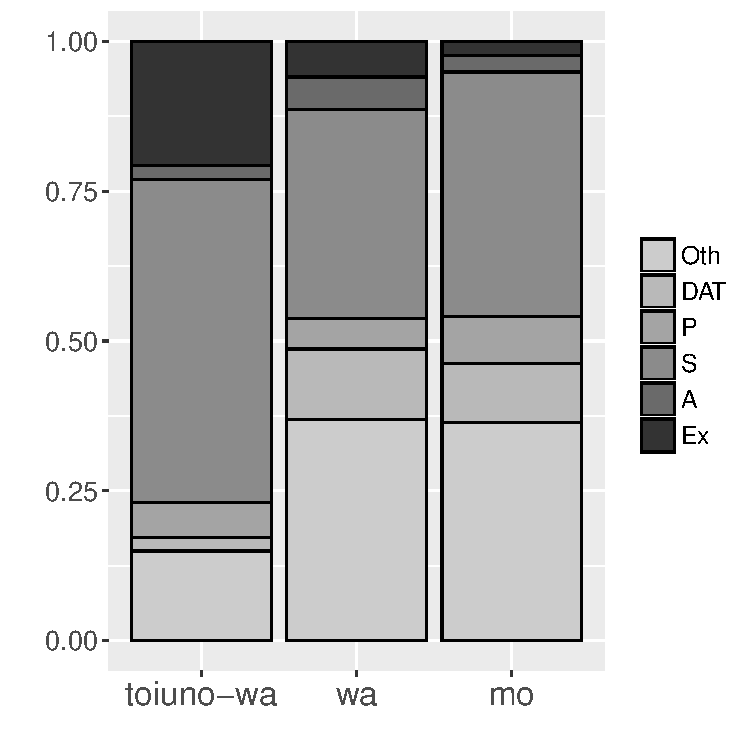
\includegraphics[width=0.5\textwidth]{figure/ASPTopPar.pdf}
	\caption{Topic markers vs.~grammatical function}
	\label{Par:ASPTopParF}
	\end{center}
%\end{minipage}
\end{figure}
\begin{figure}
%\begin{minipage}{0.5\textwidth}
	\begin{center}
	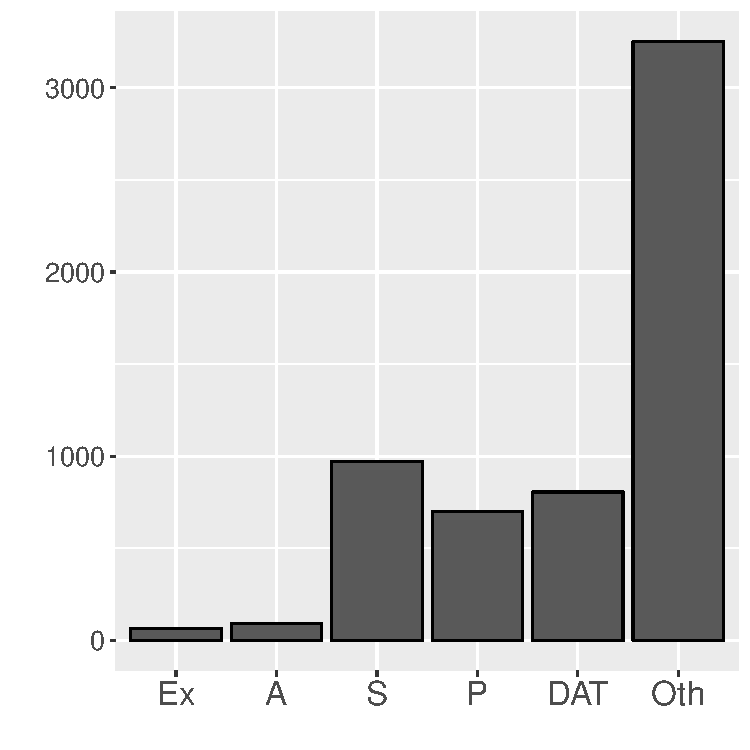
\includegraphics[width=0.5\textwidth]{figure/ASPall.pdf}
	\caption{Overall distributions of elements}
	\label{Par:ASPallF}
	\end{center}
%\end{minipage}
\end{figure}


Whereas \citeA[2]{aoki92} reported that
84.7\% of \ci{wa} attaching nouns code so-called subjects (A and S in my terms, nominative case in her terms) in novels and essays,
only 40.3\% of \ci{wa} in our data codes As and Ss,
as shown in Table \ref{Par:ASPTopParT} and Figure \ref{Par:ASPTopParF}.
This table and figure include all kinds of elements excluded in other analyses.%
 \footnote{
 Refer to \S \ref{FW:Cor:AnaRel} to see what is excluded.
 }
Figure \ref{Par:ASPallF},
which represents the overall frequencies of elements,
is shown for comparison.
This graph also includes all kinds of elements excluded in other graphs.
On the other hand, Table \ref{Par:ASPTopParT} and Figure \ref{Par:ASPTopParF} show that
59.0\% of \ci{toiuno-wa} codes so-called subjects.
This demonstrates that
\ci{toiuno-wa} in spoken Japanese is in fact closer to \ci{wa} in written Japanese
in terms of the preference of coding grammatical functions. %and the functions of spoken \ci{wa} are shifting.
Although a majority of the literature focuses on \ci{wa} coding subjects,
the results suggest that \ci{wa} codes other kinds of elements in spoken Japanese.

So-called subjects have tspecial status in the discourse;
they are interpreted as definite in the discourse
even though the NP is coded by \ci{ga} instead of \ci{wa}.
For example,
consider the difference between \Next and \NNext.
%
\ex.
 \a.[Q:] Why were you absent yesterday?
 \bg.[A:] \EM{kuruma-ga} inu-o hii-ta-n-desu \\
		car-\ci{ga} dog-\ci{o} run.over-\ab{past}-\ab{nmlz}-\ab{plt} \\
		`(My) car ran over (a) dog.'
 \bg.[A$^{\prime}$] \EM{kuruma-ga} inu-ni butukat-ta-n-desu \\
   car-\ci{ga} dog-\ab{dat} hit-\ab{past}-\ab{nmlz}-\ab{plt} \\
   `(My) car hit (a) dog.'
%			\b. My dog ate a toy.
%			\b. A toy was eaten by my dog.
	
\ex. \a.[Q:] Why were you absent yesterday?
	\bg.[A:] \EM{inu-ga} kuruma-ni hik-are-ta-n-desu \\
		dog-\ci{ga} car-\ab{dat} run.over-\ab{pass}-\ab{past}-\ab{nmlz}-\ab{plt} \\
		`(My) dog was run over by (a) car.'
 \bg.[A$^{\prime}$] \EM{inu-ga} kuruma-ni butukat-ta-n-desu \\
   dog-\ci{ga} car-\ab{dat} hit-\ab{past}-\ab{nmlz}-\ab{plt} \\
   `(My) dog hit (a) car.'
%			\b. A dog ate my toy.
%			\b. My toy was eaten by a dog.

These utterances represent the same propositional meaning
that can be paraphrased as `(a/the) car ran over (a/the) dog.'
Note that
since Japanese does not have obvious ways to code definiteness,
both `car' and `dog' can be potentially interpreted as either definite or indefinite,
and hence `car' and `dog' are expressed in the same way in \LLast and \Last
except for case markers.
Under these conditions,
the subjects `car' in \LLast and `dog' in \Last are interpreted as definite, % and are associated with the speaker,
while the non-subjects `car' in \Last and `dog' in \LLast are indefinite,
according to the author's intuition.
NPs coded by \ci{wa} are also likely to be interpreted as definite since
the referent of those NPs are assumed to be evoked.
This observation suggests that subjects without topic-marking still function like topic markers.
This is worth investigating in the future
since my argument is no more than an impressionistic analysis.


%Similarly,
%the contrast between \Next[-A2] and \Next[-A2$^{\prime}$] and  shows that
%the subject `friend' in \Next[-A2] can only be interpreted as the speaker's friend
%(if there are no other salient people in the context),
%while the object `friend' in \Next[-A2$^{\prime}$] can be interpreted as the speaker's friend or the subject Taro's friend.
%%
%\ex.
% \a.[A1:] Oh my gosh...
% \b.[B1:] What happened?
% \bg.[A2:] ima \EM{tomodati-ga} taroo nagut-ta-n-da-yo \\
%   now friend-\ci{ga} Taro hit-\ab{past}-\ab{nmlz}-\ab{cop}-\ab{fp} \\
%   `(My) friend hit Taro just now.'
% \bg.[A2$^{\prime}$:] ima \EM{taroo-ga} tomodati nagut-ta-n-da-yo \\
%   now Taro-\ci{ga} friend hit-\ab{past}-\ab{nmlz}-\ab{cop}-\ab{fp} \\
%   `Taro hit (my/his) friend just now.'
%

%%% Silversteinの名詞句階層と角田

%%----------------------------------------------------
\subsection{Hierarchy of topic-coding}\label{Par:ArgStr:TopHierarchy}

There seems to be a hierarchy of topic-coding;
given As and Ss are more likely to be coded by topic markers than given Ps.
For example, consider the following example.
In \Next,
\ci{sohu} `grandfather' is introduced in line a, and
\ci{pan} `bread' is introduced in line b.
In line c, which is of interest in the discussion,
\ci{oziityan} `grandfather' is coded by \ci{wa}, but
\ci{sore} `that', which refers to the bread in line b, is coded by the case particle \ci{o}.
%
\ex.
 \ag. uti-no \EM{sohu}-tteiuno-ga okasi-ga sukina mono-de \\
 		out-\ab{gen} grandfather-\ci{toiuno}-\ci{ga} sweet-\ci{ga} favorite thing-\ab{cop} \\
		`Our grandfather likes sweets.'
 \bg. yoku pan-ya-san-de \EMi{kasi-pan}-o kat-te kuru-n-desu-ga \\
   often bread-store-\ab{hon}-\ab{loc} sweet-bread-\ci{o} buy-and come-\ab{nmlz}-\ab{cop}.\ab{plt}-though \\
   `(He) often buys sweet bread and comes home,'
 \bg. e n \EMi{sore-o} i maa yoowa \EM{oziityan-wa} issyookenmee taberu-n-desu-keredomo \\
   \ab{fl} \ab{frg} that-\ci{o} \ab{frg} \ab{fl} in.a.word grandfather-\ci{wa} trying.best eat-\ab{nmlz}-\ab{cop}.\ab{plt}-though \\
   `that, he tries his best to eat it, but'
 \b. he cannot eat all and
 \b. gives leftovers to the dog...
  \hfill{(\code{S02M0198: 244.48-262.82})}

It is unnatural for \ci{wa} to code \ci{sore} referring to the bread
instead of \ci{oziityan} `grandfather',
as shown in \Next[c$^{\prime}$].
If A (e.g., \ci{obaatyan} `grandmother') is newly introduced, as in \Next[c$^{\prime\prime}$],
there is no problem for \ci{wa} coding \ci{sore};
\ci{obaatyan} `grandmother' is naturally coded by \ci{ga} instead of \ci{wa}.
%
\ex.
 \ag.[c$^{\prime}$.] e n \EMi{sore-\{o/wa\}} i maa yoowa ??\EM{oziityan-ga} issyookenmee taberu-n-desu-keredomo \\
   \ab{fl} \ab{frg} that-\{\ci{o}/\ci{wa}\} \ab{frg} \ab{fl} in.a.word grandfather-\ci{ga} trying.best eat-\ab{nmlz}-\ab{cop}.\ab{plt}-though \\
   `that, my grandfather tries his best to eat it, but...'
  \bg.[c$^{\prime\prime}$.] e n \EMi{sore-\{o/wa\}} i maa yoowa \EM{obaatyan-\{ga/??wa\}} issyookenmee taberu-n-desu-keredomo \\
   \ab{fl} \ab{frg} that-\{\ci{o}/\ci{wa}\} \ab{frg} \ab{fl} in.a.word grandmother-\ci{ga}/\ci{wa} trying.best eat-\ab{nmlz}-\ab{cop}.\ab{plt}-though \\
   `that, my grandmother tries her best to eat it, but...'
   \hfill{(modified from \Last[c])}

In fact, the majority of anaphoric Ps are still coded by \ci{o},
instead of topic markers,
whereas a higher ratio of anaphoric As and Ss are coded by topic markers.
Tables \ref{Par:ASPParGivenT} and \ref{Par:ASPParNewT} and
Figures \ref{Par:ASPParGivenF} and \ref{Par:ASPParNewF} show
the distribution of topic and case markers coding A, S, and P.
Table \ref{Par:ASPParGivenT} and Figure \ref{Par:ASPParGivenF} represent the distribution of topic and case markers coding anaphoric A, S, and P.
As the table and the graph show,
while 44.1\% of anaphoric As and 38.8\% of anaphoric Ss are coded by topic markers,
only 8.4\% of anaphoric Ps are coded by topic markers.
On the other hand,
the majority of non-anaphoric elements are coded by case markers,
although non-anaphoric Ss (most of which are in fact inferable) are remarkably more often coded by \ci{wa} than others.

I propose the hierarchy \Next for topic-coding.
The given elements higher in this hierarchy are more likely to be coded by topic markers.
%
\ex.\label{ASPGivenSchema}
 A, S $>$ P

The hierarchy indicates that so-called subjects are more likely to be coded by topic markers.
This hierarchy is a topic hierarchy:
the hierarchy of elements which are more likely to be topics \cite{givon76,keenan76,comrie79,comrie83,dubois87}.
%%% あやしい
This hierarchy is present in many languages in various ways.
For example, A and S are more likely to agree with the verb than P cross-linguistically.
Also, A and S are more likely to be zero-coded than P.
Japanese \ci{wa}-coding seems to follow this hierarchy;
if there are two given elements potentially coded by \ci{wa},
A and S are preferred over P following the hierarchy in \Last.

\begin{table}
\begin{center}
\tblcaption{Markers for anaphoric}
\label{Par:ASPParGivenT}
\begin{tabular}{lrrrr}
	\toprule
	              & Ex & A & S & P \\
	\midrule
	 Topic marker & 20 & 15 & 97 & 15 \\
	              & \rt{(100\%)} & \rt{(44.1\%)} & \rt{(38.8\%)} & \rt{(8.4\%)} \\
	 Case marker  & 0 & 19 & 153 & 163 \\
	              & \rt{(0\%)} & \rt{(55.9\%)} & \rt{(61.2\%)} & \rt{(91.6\%)} \\
	\midrule
	 Sum          & 20 & 34 & 250 & 178 \\
%	              & \rt{(100\%)} & \rt{(100\%)} & \rt{(100\%)} & \rt{(100\%)} \\
	\bottomrule
%             Ex   A   S   P DAT
%  toiuno-wa   9   1  26   2   0
%  wa          11  14  71  13   0
%  ga          0  19 153   0   0
%  o           0   0   0 163   0
\end{tabular}
\end{center}
\end{table}

\begin{table}{}
\begin{center}
\tblcaption{Markers for non-anaphoric}
\label{Par:ASPParNewT}
\begin{tabular}{rrrr}
	\toprule
	 Ex & A & S & P \\
	\midrule
	 12 & 1 & 74 & 13 \\
	 \rt{(100\%)} & \rt{(8.3\%)} & \rt{(21.6\%)} & \rt{(6.8\%)} \\
	 0 & 11 & 269 & 177 \\
	 \rt{(0\%)} & \rt{(91.7\%)} & \rt{(78.4\%)} & \rt{(93.2\%)} \\
	\midrule
	 12 & 12 & 343 & 190 \\
%	 \rt{(100\%)} & \rt{(100\%)} & \rt{(100\%)} & \rt{(100\%)} \\
	\bottomrule
%             Ex   A   S   P DAT
%  toiuno-wa   8   1  16   3   0
%  wa          4   0  58  10   0
%  ga          0  11 269   0   0
%  o           0   0   0 177   0
\end{tabular}
\end{center}
\end{table}

\begin{figure}
%\begin{minipage}{0.5\textwidth}
	\begin{center}
	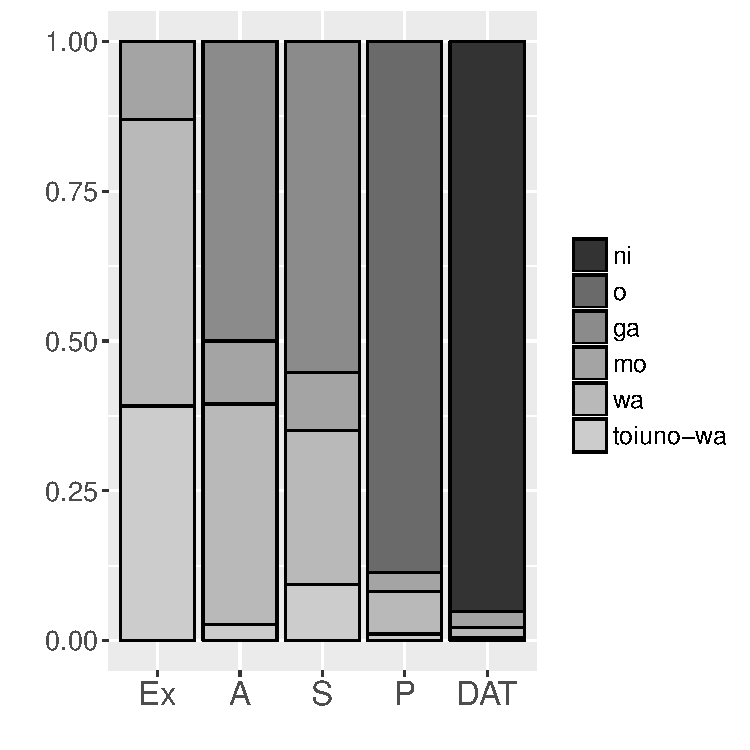
\includegraphics[width=0.5\textwidth]{figure/ASPParGiven.pdf}
	\caption{Markers for anaphoric}
	\label{Par:ASPParGivenF}
	\end{center}
\end{figure}
\begin{figure}
%\end{minipage}
%\begin{minipage}{0.5\textwidth}
	\begin{center}
	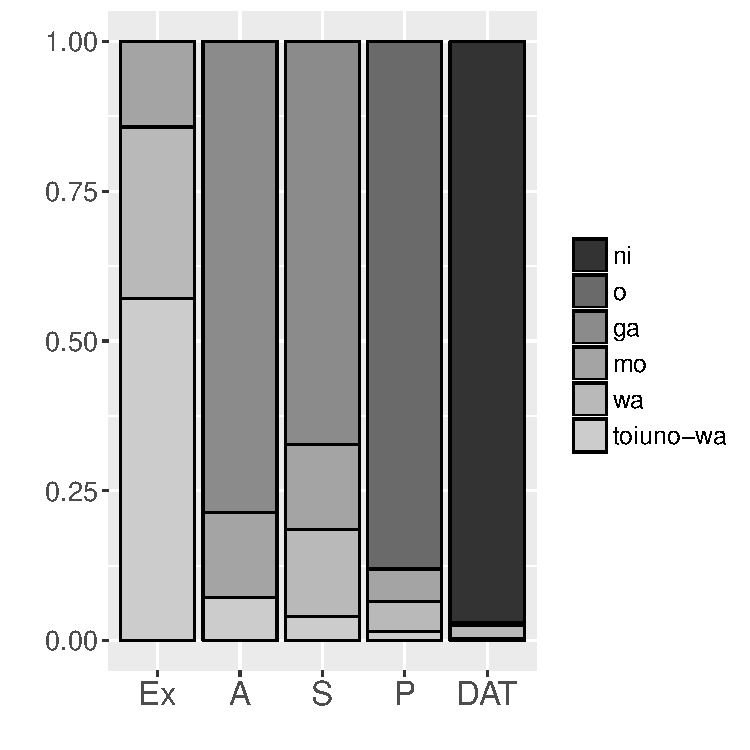
\includegraphics[width=0.5\textwidth]{figure/ASPParNew.pdf}
	\caption{Markers for non-anaphoric}
	\label{Par:ASPParNewF}
	\end{center}
%\end{minipage}
\end{figure}


%%----------------------------------------------------
\subsection{Ex or detached NPs}\label{Par:Subj:Ex}

Finally, I discuss associations between ``Ex'' and topic markers.
In \S \ref{FW:Cor:TopFoc},
Ex was defined as elements ``which appear to be part of the clause but do not have direct relationships with the predicate'' (p.~\pageref{FW:Cor:TopFoc:ExDef}).
A typical example is shown in \Next.
In \Next, the predicate \ci{nagai} `long' is directly related to \ci{hana} `nose'.
\ci{Zoo} `elephant' is not directly related to the predicate;
it is not the elephant itself that is long.
%
\exg. \EM{zoo-wa} hana-ga nagai \\
		elephant-\ci{wa} nose-\ci{ga} long \\
		`The elephant, the nose is long (The elephant has a long nose).' \hfill{\cite{mikami60}}

Tables \ref{Par:ASPParGivenT} and \ref{Par:ASPParNewT} and
Figures \ref{Par:ASPParGivenF} and \ref{Par:ASPParNewF}
show that Ex is only coded by topic markers.
Tables \ref{Par:ASPTopParT} and Figures \ref{Par:ASPTopParF}
show that 21.7\% of \ci{toiuno-wa}-coded elements and
5.9\% of \ci{wa}-coded elements are categorized into Ex.

\citeA{lambrecht94}
discusses cross-linguistic cases of Ex (in his term, ``detached'' topic)
and argues that
``in some languages at least, the detached topic NP cannot be a constituent [...] of the clause with which it is pragmatically associated'' (p.~192).
In \Next, examples in English,
the detached topics are not constituents of the clause;
rather, they have a part-whole relation with some element(s) within a clause.
In \Next[a], the detached topic \ci{the typical family today} is not a constituent of the clause;
instead, it is associated with \ci{the husband and the wife} pragmatically.
In the same way, the detached topics \ci{tulips} in \Next[b] and
\ci{other languages} in \Next[c]
are pragmatically associated with constituents of the clauses \ci{bulbs} and \ci{tones}, respectively.
%
\ex.
% \a. (Six year old girl, explaining why the African elephant has bigger ears than Asian elephant) \\
%  \EM{The African elephant}, it's so hot there, so \EM{he} can fan himself.
 \a. (From a TV interview about the availability of child care) \\
   That isn't the typical family anymore.
   \EM{The typical family today},
   \EMt{the husband and the wife} both work.
 \b. (Talking about how to grow flowers) \\
   \EM{Tulips}, you have to plant new \EMt{bulbs} every year?
 \b. (Lecture in an introductory linguistics course) \\
   \EM{Other languages}, you don't just have straight \EMt{tones} like that.
% \b. (From an article in the San Fransisco Chronicle about a wealthy town in Dade Country, Florida, becoming a ``'fort against crime') \\
%   ``what we are trying to do here is keep this community what it is, a beautiful, safe place to live,'' said police chief Dick de Stefani.
%   ``\EM{Dade Country}, you just can't belive the rise in crime.''
  \b.[] \hfill{\cite[193]{lambrecht94}}

These detached topics are strikingly similar to
``Ex'' in Japanese.

Lambrecht also discusses cases in which
topics are not counted as constituents of the clause
even though they appear to be constituents.
German, for example, has the principle that only allows the verb in the second position within a clause, as exemplified in \Next[a-d].
However, the detached topic constituents that appear at the beginning are not counted as the first constituent of the clause.
%rather they are outside of the clause.
As exemplified in \Next[e],
the verb \ci{isst} `ate' appears in the second position assuming that the preceding \ci{den} `it' is in the first position,
which indicates that
the detached topic \ci{den Apfel} is not counted as the first constituent in the clause.
In fact, as in \Next[f],
it is unacceptable
if the detached topic \ci{den Apfel} is counted as the first constituent.%
 \footnote{
 \chd{\ci{Apfel} `apple' in e, f of \ref{Par:Subj:Ex:Ex:Apfel} is considered to be ``detached'' because
 the resumptive pronoun \ci{den} `it.\ab{acc}' is regarded as argument of the clause and \ci{Apfel} itself does not function as argument.}
 }
%
\ex.\label{Par:Subj:Ex:Ex:Apfel}
 \ag. Hans \EM{isst} den Apfel. \\
   Hans eat the.\ab{acc} apple \\
   `Hans eats the apple.' \hfill{(SVO)}
 \b. Den Apfel \EM{isst} Hans. \hfill{(OVS)}
 \b. *Den Apfel Hans \EM{isst}.\hfill{(*OSV)}
 \bg. Den isst Hans. \\
   it.\ab{acc} eat Hans \\
   `Hans eats it.' \hfill{(OVS)}
 \bg. \EMi{Den} \EMi{Apfel} den \EM{isst} Hans. \\
   the.\ab{acc} apple it.\ab{acc} eat Hans \\
   `The apple, Hans eats it.'  \hfill{(TOVS)}
 \b. *\EMi{Den} \EMi{Apfel} \EM{isst} Hans den. \hfill{(*TVSO)}
 \b.[] \hfill{(op.cit.: 194)}

Both the topicalized NP \ci{den Apfel} and the resumptive pronoun \ci{den} in \Last[e] appear as accusative.
According to Lambrecht, however,
it is optional for the topicalized NP,
while it is obligatory for the resumptive pronoun.
This is also reminiscent of topic-marking in Japanese.
In Japanese,
nominative and accusative codings are overridden by topic-marking
and the case for A, S, and P coded by topic markers are not overtly expressed
as has been discussed in \S \ref{Back:GeneralChar:Wa}.
%Whereas the detached topic \ci{den Apfel} in the examples above have the coreferent pronoun \ci{den} within the clause,
%He discusses cases where the detached topics do not have the coreferent in the clause:
%examples of unlinked topic construction.


The fact that topics tend to be ``detached'' from the predicate and
lose case marking cross-linguistically suggests the possibility that
there are some universal motivations behind this phenomenon.
I argue that at least one of the motivations is clause-chaining.
In clause-chaining,
the speaker combines multiple clauses to form a thematic unit
\cite{longacre85,martin92,givon01}.
\Next is an example of clause-chaining.
%
\ex. She came in, [\O] stopped, [\O] looked around and froze.\\
     \hfill{\cite[349]{givon01}}

By combining clauses in this way,
thematic continuity is achieved.
In clause-chaining,
the detached topic, which typically appears utterance-initially, as will be discussed in Chapter \ref{WordOrder},
is not necessarily an argument of the clauses;
instead, it is pragmatically related to the following clauses.
For example, in \Next,
where the speaker talks about a life in Iran,
\ci{mukoo-no hito} `people there (in Iran)' in \Next[a] is detached
and annotated as ``Ex''
because its predicate \ci{hukaku} `deep', which has a part-whole relations with the people, has the so-called subject \ci{hori} `(face) form'.
In \Next[b-c], the speaker continues to talk about her
by clause-chaining.
\ci{Kodomo} `child' in \Next[c] also has a part-whole relation
with the Iran people.
%
\ex.
 \ag. eto n \EM{mukoo-no} \EM{hito-toiuno-wa} hontooni \EMi{hori-ga} hukaku-te \\
      \ab{fl} \ab{fl} there-\ab{gen} person-\ci{toiuno-wa} really form-\ci{ga} deep-and \\
      `People there (in Iran), (their) face forms are really chiseled,'
 \bg. kiree-de \\
      beautiful-and \\
      `beautiful,'
 \bg. \EMi{kodomo-nanka-wa} anoo sugoku kawaii kao-o si-tei-mashi-ta \\
      child-\ab{hdg}-\ci{wa} \ab{fl} very cute face-\ci{o} do-\ab{prog}-\ab{plt}-\ab{past} \\
      `children had very cute faces.'
      \src{S03F0072: 375.01-386.35}
%S03F0072|00375010L|375.010443|386.346614|L|(F えと)(D ん)(0.507)向こうの人というのは本当に(F あのー)彫りが深くて(0.229)奇麗で(0.907)(F えーと)子供なんかは(0.587)(F あのー)凄く(1.012)かわいい顔をして(0.627)いました|[文末]|

Clause-chaining is a useful way to talk about something;
the speaker puts the topic at the beginning and
continues to describe the topic as much as s/he can.
In the descriptions in clause-chaining,
the topic is not necessarily an argument;
it is pragmatically associated with each clause.
The hearer does not get lost.
The hearer can trace the topic
when the speaker provides enough evidence
through linguistic expressions (such as particles, word order, and intonation) and other means (such as gesture, background knowledge, sequence of conversation, etc.).

\citeA[Chapter 2]{mikami60} points out that
\ci{wa}-coded NPs can ``go beyond periods'' (p.~117) and ``commas'' (p.~130).
This is closely related to what I argue here.
%
%\ex.
% \ag. \EM{tookyoo-wa} kinbenna hito-ga takusan i-te \\
% \bg. issyookenmee hatarai-teiru-no-da-ga \\
% \bg. mati-mo kitanai-si \\
% \bg. miti-mo kitanai \\
%
He states:
``in general, `X-\ci{wa}', skipping adverbial clauses in the middle, governs the final main clause.
However, it [sometimes] governs the verbs in the middle a little bit;
this is what I call [\ci{wa}'s] going beyond commas'' (p.~130).
Of course, there are no commas and periods in spoken language,
\ci{wa} and \ci{toiuno-wa} go beyond ``commas'' and ``periods'' by governing the whole clause-chaining.
%In \S \ref{Back:GeneralChar:Wa},

%%----------------------------------------------------
%%----------------------------------------------------
\section{Discussion}\label{ParticlesDiscussion}

%%----------------------------------------------------
\subsection{Distribution of markers and semantic space}

\begin{figure}
%\begin{minipage}{0.5\textwidth}
	\begin{center}
	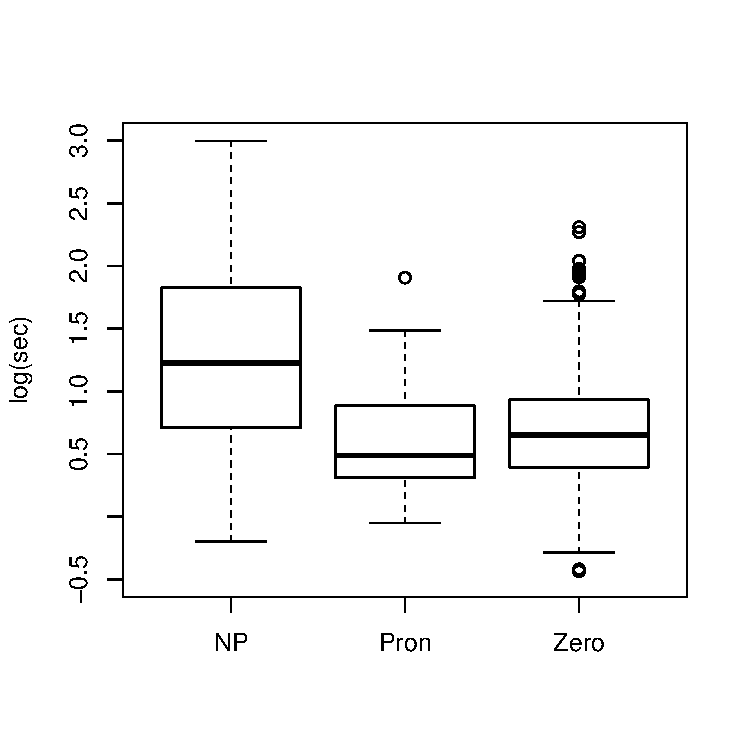
\includegraphics[width=0.5\textwidth]{figure/DistExpType.pdf}
	\caption{Anaphoric distance vs.\ expression type (all)}
	\label{DistExpTypeF2}
	\end{center}
%\end{minipage}
%\begin{minipage}{0.5\textwidth}
%	\begin{center}
%	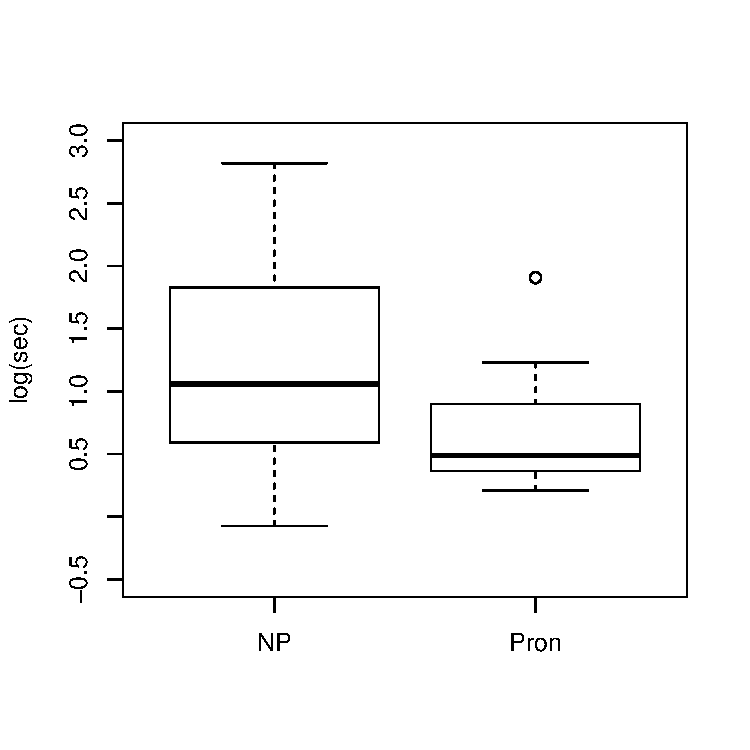
\includegraphics[width=0.99\textwidth]{figure/DistExpTypeTop.pdf}
%	\caption{Anaphoric distance vs.\ expression type (coded by topic markers)}
%	\label{DistExpTypeParF}
%	\end{center}
%\end{minipage}
\end{figure}

As discussed in \S \ref{ParIntro},
the particles code elements with features that can be mapped onto a conceptual space.
As reflected in Table \ref{ParInfoStatusT} and discussion in \S \ref{TopPar},
topic markers map onto a conceptual space of the given-new taxonomy,
while, as in Table \ref{OvertZeroCaseParT1} and discussion in \S \ref{CasePar},
case markers map onto a conceptual space of agentivity, focushood, contrastiveness, and possibly animacy.

The semantic map of topic markers in Japanese indicates that
inferable and evoked statuses form a connected region and are expressed by the same marker \ci{wa},
while declining and unused statuses form a connected region and are expressed by the same marker (a copula followed by \ci{kedo} or \ci{ga});
hence, the inferable status is closer to the evoked status, and the declining status is closer to unused in the conceptual space.
This makes sense because inferable elements are more relevant to
the current topic than declining elements.
For example, in \Next,
the inferable element \ci{gen'in} `cause' is coded by \ci{wa}.
The element `cause' is inferable because the disease has been already introduced and the cause of the disease can be considered to be part of the knowledge of getting a disease.
%
\ex.
 \a. (The speaker got a rare disease.)
 \b. First I visited several local hospitals.
 \b. I was examined several times, but
 \bg. \EM{gen'in-wa} humee-de \\
   cause-\ci{wa} unclear-\ab{cop} \\
   `the cause (of the disease) was unclear.'
   \hfill{(\code{S02F0010: 74.93-82.60})}
%
%まず地元の病院のを何軒か回りました
%でその度に検査をして
%あの調べたんですが
%原因は不明で (S02F0010: 74.93-82.60)

In \Last,
the cause of the disease is relevant to the current topic, i.e., the speaker's disease.
Later in this speech,
the speaker talks about her parents and friends;
in this case the cause of the disease is considered to be declining and is less relevant to the current topic (her parents and friends).
Declining elements like the cause of the disease become unused as the time passes.
If the speaker brings up the cause of the disease two days later,
she will code it as unused.
Thus, I argue that the adjacency of inferable and evoked statuses and that of declining and unused statuses are cognitively motivated and I argue that this is universal.

Moreover,
I propose that there are at least two kinds of evoked status:
evoked and what I call strongly evoked.
Evoked elements are full NPs, and
strongly evoked elements are zero and overt pronouns.
%Active elements are, as I have discussed so far,
%coded by \ci{toiuno-wa} and \ci{wa}.
%Strongly active elements are, on the other hand, so-called zero pronouns.
%Zero pronouns are more active than elements coded by \ci{toiuno-wa} and \ci{wa}.
Figure \ref{DistExpTypeF2} shows the time difference (anaphoric distance) on a logarithmic scale between when the first mora of the element in question is produced and when that of its antecedent is produced.
Zero pronouns are assumed to be produced at the time when
the first mora of the predicate is produced.
The anaphoric distance approximates activation cost;
smaller distance indicates lower activation cost,
while larger distance indicates higher activation cost.
Figure \ref{DistExpTypeF2} represents the anaphoric distance of three kinds of elements:
full NPs, pronouns, and zero pronouns.
%Figure \ref{DistExpTypeParF} indicates the distance of elements coded by \ci{toiuno-wa} and \ci{wa}.
As is clear from the figure,
the anaphoric distance of zero and overt pronouns is smaller than
that of NPs,
which indicates that
zero and overt pronouns are more evoked than full NPs \chd{(fixed effects model, $p < 0.001$)}.
Therefore, I propose the status called ``strongly evoked''.
I add this status in Table \ref{ParInfoStatusT2}.
Since overt pronouns coded by the topic markers are as strongly evoked as zero pronouns,
I suppose that the topic markers \ci{wa} and \ci{toiuno-wa} can also code strongly evoked elements.
%%% Strongly activeだったら、トイウノハとハも付ける

Markers for focus coding map onto agentivity, focushood, contrastiveness, and possibly animacy
as has been discussed in \S \ref{CasePar}.
Table \ref{OvertZeroCaseParT} in \S \ref{CasePar} indicates that
A and agent S are adjacent to each other, and
patient S and P are adjacent.
This makes sense because
A is conceptually closer to agent S, and
P is conceptually closer to patient P.
%I will discuss other features such as focushood and animacy in the following section.

\begin{table}[hbt]
	\caption{Topic marker vs.\ activation status and the given-new taxonomy}
	\label{ParInfoStatusT2}
\fittable{
	\begin{tabular}{|l|l|c|c|}
	\hhline{----}
	Activation status & Given-new taxonomy & Topic & Focus \\
	\hhline{|-|-|-|-|}
	                 &        & Zero pronoun  & -- \\
	\hhline{|~|~|~|-|}
	 Strongly active & Evoked & Overt pronoun &  \\
	                 &        & \ci{toiuno-wa, wa}, {\O} &  \\
	\hhline{|-|-|-|~|}
	 Active & Evoked & \ci{toiuno-wa, wa}, {\O} &  \\
	\hhline{|-|-|-|~|}
	\cellcolor[gray]{.9}Semi-active & \cellcolor[gray]{.9}Inferable & \ci{wa}, {\O} & case markers, {\O} \\
	\hhline{|-|-|-|~|}
	 Semi-active & Declining & \multirow{2}{*}{\ab{cop}-\ci{kedo/ga}, {\O}}  &  \\
	\hhline{|-|-|~|~|}
	\cellcolor[gray]{.9}Inactive & \cellcolor[gray]{.9}Unused &  &  \\
	\hhline{|-|-|-|~|}
	\cellcolor[gray]{.9}Inactive & \cellcolor[gray]{.9}Brand-new &  --  &  \\
%	\rowcolor{gray}
%	 & (Anchored) & & \\
%	\rowcolor{gray}
%	inactive & Brand-new &  --  & case markers, {\O} \\
%	\rowcolor{gray}
%	 & (Unanchored) & & \\
	\hhline{----}
	\end{tabular}
}
\end{table}

%%----------------------------------------------------
\subsection{Distribution of markers and markedness}\label{Par:Dis:Markedness}

As discussed in \S \ref{CasePar} and summarized in Table \ref{OvertZeroCaseParT},
the distinction between overt vs.\ zero particles for focus coding is sensitive to grammatical functions, contrastiveness, and animacy.
%while that for topic coding is sensitive to activation status and contrastiveness as discussed in \S \ref{TopPar}.
The distribution of overt vs.\ zero particles for non-contrastive focus coding in Table \ref{OvertZeroCaseParT}
is similar to that of split intransitive languages,
if one ignores \ci{ga}-coding for patient S.
In general, split intransitive languages code S differently
depending on whether it is an agent or a patient;
agent S is coded in the same way as A in the transitive clause,
while patient S is coded in the same way as P.
\Next shows examples from Georgian.%
	\footnote{
	Examples are from the handouts in the lecture called Typology and Universals given by Matthew Dryer at the University at Buffalo in 2010.
	Glosses are modified.
	}
\ex. Georgian, South Caucasian
	\ag. \tp{vano-\EMi{m}} \tp{gamozarda} \tp{Zma-\EMi{\O}} \\
		Vano-\ab{a} \ab{3}.\ab{3}.grow brother-\ab{p} \\
		`Vano raised his brother.' \hfill{(A \& P)}
	\bg. \tp{vano-\EMi{m}} \tp{imGera} \\
		Vano-\ab{a} 3.sing \\
		`Vano sang.' \hfill{(Agent S)}
%	\bg. \tp{bav\v{s}v-ma} \tp{i{\.*t}ira} \\
%		child-\ab{act} 3.cry \\
%		`The child cried.' \hfill{(agent S)}
	\bg. \tp{rezo-\EMi{\O}} \tp{gamoizarda} \\
		Rezo-\ab{p} 3.grow \\
		`Rezo grew up.' \hfill{(Patient S)}
%
%\ex. Choctaw
%	\ag. \tp{alla-t} \tp{ofi} \tp{poshohli-tok} \\
%		child-\ab{nom} dog rub-\ab{past} \\
%		`The child patted the dog.' \hfill{(A \& P)}
%	\bg. \tp{hattak-a-t} \tp{oho:yo} ahpali-tok \\
%		man-\ab{det}-\ab{nom} woman kiss-\ab{past} \\
%		`The man kissed the woman.' \hfill{(A \& P)}
%	\bg. \tp{katos-a-t} \tp{\~{\i}pa-tok} \\
%		cat-\ab{det}-\ab{nom} eat-\ab{past} \\
%		`The cat ate.' \hfill{(agent S)}

Spoken Japanese and Georgian in \Last follow the typological tendency that
agent S and A tend to be overtly coded,
while patient S and P tend to be zero-coded.
%%% 文献
On the other hand,
Spoken Japanese does not follow the tendency of nominative/accusative languages:
the tendency that A and S (nominative elements) are more likely to be zero-coded than P (accusative elements).
I argue that, in coding focus elements,
patient elements are ``unmarked'',
i.e., more frequent than agent elements,
and are more likely to be zero-coded than agent elements.
This is supported by studies such as \citeA{dubois87} and \citeA{duboisetal03}.
On the other hand,
in coding topic elements,
agent elements are more frequent than patient elements,
and are more likely to be zero-coded than patient elements.
This is observed in another dialect of Japanese: Kansai Japanese.
In Kansai Japanese,
contrastive topic agents (A and agent S) can be zero-coded,
while contrastive topic patients (P and patient S) are overtly coded,
which is summarized in Table \ref{DistPartTopKJ}.
See \citeA{nakagawa13m}
for more detailed discussion on the relation
between markedness and the distribution of zero vs.\ overt particles in Standard and Kansai Japanese.

\begin{table}
\begin{center}
	\caption{Contrastive-topic coding in Kansai Japanese}
	\label{DistPartTopKJ}
\begin{tabular}{lcccc}
	\toprule
	 & A & \multicolumn{2}{c}{S} & P \\
\cline{3-4}
			 & & agent & patient & \\
	\midrule
%	inactive Topic & \cellcolor[gray]{.9} {\O} & \cellcolor[gray]{.9} {\O}  & \cellcolor[gray]{.9} {\O} & \cellcolor[gray]{.9} {\O} \\
%%	\rowcolor[gray]{0.95}
%	Activated Topic & \cellcolor[gray]{.9} {\O} & \cellcolor[gray]{.9} {\O}  &  \cellcolor[gray]{.9} {\O} & \cellcolor[gray]{.9} {\O} \\
%%	Activated Topic (SJ) & {\O}/\ci{wa} & {\O}/\ci{wa} & {\O}/\ci{wa} & {\O}/\ci{wa} \\
%%	\rowcolor[gray]{0.95}
	Contrastive Topic & {\O}/\ci{wa}  & {\O}/\ci{wa} & \ci{wa} & \ci{wa} \\
%	Contrastive Topic (SJ)  & \ci{wa} & \ci{wa} & \ci{wa} & \ci{wa} \\
	\bottomrule
\end{tabular}
\end{center}
\end{table}

As has been discussed in \S \ref{Par:CasePar:Ga:GaFoc},
\ci{ga} sometimes codes non-nominative focus NPs.
The theory of markedness also gives a hint to explain why \ci{ga} is on the way to grammaticalize into a focus particle;
focus A is the most rare in natural occurring discourse
and it is likely for Japanese native speakers to associate the marker \ci{ga} with focushood.
On the other hand, P is very frequently focused,
in which case, it is less likely to associate the marker \ci{o} with focushood.


%%%----------------------------------------------------
%\subsection{Continuity between topic and focus}\label{Par:Dis:Cont}


%%----------------------------------------------------
%%----------------------------------------------------
\section{Summary}

%%----------------------------------------------------
\subsection{Summary of this chapter}

This chapter discussed the distributions of so-called topic marker and case markers in Japanese.
I argued that
different markers are sensitive to different features, and
at the same time,
 multiple features contribute to the usage of a single marker.


%%----------------------------------------------------
\subsection{Remaining issues}

While there are many remaining issues,
one of the biggest issues is that
it is necessary to test the proposals in this chapter through other empirical methods.
If the proposals are supported also by other methods,
they become more sound.
In particular, the distribution of the zero particles is mainly based on a few native speakers' acceptability judgements.
This should be tested with a larger number of native speakers.
One possible experiment is to ask subjects to listen to short conversation where the particles in question are blurred
and to produce what they hear.
This is easier than subtle acceptability judgements and linguistically na\"{\i}ve subjects can also participate in it.

Another issue is the focus test.
So far we only have the \ci{hee} test and the \ci{no} test,
which depend on the author's acceptability judgements.
One possible experiment is to ask subjects to listen to speech used in this study
and respond to what the speaker means by \ci{hee}
as if they were the hearers.
The elements that many subjects respond to are more likely to be foci.
Another possibility is to investigate conversations and study the elements that the hearer actually responds to.
\citeA{denetal12} annotated response tokens like \ci{hee} and the elements those response tokens address.
One might be able to use this annotation to test the second hypothesis.

